%=====================================================================
%  Simulando Qubits com PySCF: Uma Jornada do Zero aos Pontos
%  Quanticos para Computacao Quantica
%  Autor: Cristiano Alves
%
%  ARQUIVO PRINCIPAL. O conteudo esta dividido em tex/:
%     tex/preambulo.tex ... pacotes, cores, caixas didaticas, comandos
%     tex/capa.tex ........ folha de rosto
%     tex/prefacio.tex .... textos pre-textuais
%     tex/parteN.tex ...... aberturas das partes
%     tex/capNN_*.tex ..... um arquivo por capitulo
%
%  Compile com:
%      latexmk -pdf Livro_PySCF.tex
%  ou  pdflatex Livro_PySCF.tex  (2x, para sumario/referencias)
%=====================================================================

%=====================================================================
%  Simulando Qubits com PySCF: Uma Jornada do Zero aos Pontos
%  Quanticos para Computacao Quantica
%  Autores: Cristiano da Costa Alves
%           Nilseia Aparecida Barbosa
%           Fernando Manuel Araujo Moreira
%
%  Arquivo principal do livro. Compile com:
%      latexmk -pdf Livro_PySCF.tex
%  ou  pdflatex Livro_PySCF.tex  (2x, para sumario/referencias)
%=====================================================================
\documentclass[11pt,a4paper,openany]{book}

%--------------------- Codificacao e idioma --------------------------
\usepackage[utf8]{inputenc}
\usepackage[T1]{fontenc}
\usepackage[brazil]{babel}
\usepackage{lmodern}
\usepackage[zerostyle=b,scaled=.85]{newtxtt} % monospace legivel
\usepackage{microtype}

%--------------------- Matematica e graficos -------------------------
\usepackage{amsmath,amssymb,amsfonts}
\usepackage{mathtools}
\usepackage{graphicx}
\usepackage{booktabs}
\usepackage{multirow}
\usepackage{array}
\usepackage{enumitem}

%--------------------- Layout de pagina ------------------------------
\usepackage{geometry}
\geometry{left=3cm,right=2.5cm,top=2.8cm,bottom=2.8cm}
\usepackage{emptypage}
\linespread{1.05}

%--------------------- Cabecalhos ------------------------------------
\usepackage{fancyhdr}
\pagestyle{fancy}
\fancyhf{}
\fancyhead[LE]{\small\itshape\nouppercase{\leftmark}}
\fancyhead[RO]{\small\itshape\nouppercase{\rightmark}}
\fancyfoot[C]{\thepage}
\renewcommand{\headrulewidth}{0.4pt}

%--------------------- Cores -----------------------------------------
\usepackage{xcolor}
\definecolor{azulpyscf}{RGB}{18,72,120}
\definecolor{azulclaro}{RGB}{232,240,248}
\definecolor{cinzacodigo}{RGB}{247,247,247}
\definecolor{verdecom}{RGB}{60,120,60}
\definecolor{roxokw}{RGB}{140,40,140}
\definecolor{laranjastr}{RGB}{170,80,20}
\definecolor{verdeok}{RGB}{20,110,60}
\definecolor{vermelhoaviso}{RGB}{150,30,30}

%--------------------- Capitulos estilizados -------------------------
\usepackage[Sonny]{fncychap}
\ChNameVar{\Large\sffamily\bfseries\color{azulpyscf}}
\ChNumVar{\Huge\sffamily\bfseries\color{azulpyscf}}
\ChTitleVar{\Large\sffamily\bfseries\color{azulpyscf}}

%--------------------- Codigo Python (listings) ----------------------
\usepackage{listings}
\lstset{
  basicstyle=\ttfamily\small,
  keywordstyle=\color{roxokw}\bfseries,
  commentstyle=\color{verdecom}\itshape,
  stringstyle=\color{laranjastr},
  numberstyle=\tiny\color{gray},
  numbers=left,
  numbersep=8pt,
  backgroundcolor=\color{cinzacodigo},
  frame=single,
  rulecolor=\color{gray!40},
  framesep=6pt,
  breaklines=true,
  showstringspaces=false,
  tabsize=4,
  columns=fullflexible,
  keepspaces=true,
  inputencoding=utf8,
  extendedchars=true,
  literate=%
    {á}{{\'a}}1 {é}{{\'e}}1 {í}{{\'i}}1 {ó}{{\'o}}1 {ú}{{\'u}}1
    {Á}{{\'A}}1 {É}{{\'E}}1 {Í}{{\'I}}1 {Ó}{{\'O}}1 {Ú}{{\'U}}1
    {â}{{\^a}}1 {ê}{{\^e}}1 {ô}{{\^o}}1 {Â}{{\^A}}1 {Ê}{{\^E}}1
    {ã}{{\~a}}1 {õ}{{\~o}}1 {Ã}{{\~A}}1 {Õ}{{\~O}}1
    {à}{{\`a}}1 {ç}{{\c c}}1 {Ç}{{\c C}}1 {º}{{\textordmasculine}}1
    {ª}{{\textordfeminine}}1
}
\lstdefinestyle{python}{language=Python}
\lstdefinestyle{console}{
  language=bash,
  numbers=none,
  keywordstyle=\color{black},
  backgroundcolor=\color{black!88},
  basicstyle=\ttfamily\small\color{white},
  frame=single,
  rulecolor=\color{black},
}

%--------------------- Caixas didaticas ------------------------------
\usepackage[most]{tcolorbox}

\newtcolorbox{caixanota}{
  colback=azulclaro, colframe=azulpyscf, coltitle=white,
  fonttitle=\bfseries\sffamily, title=Nota,
  boxrule=0.6pt, arc=2pt, left=6pt,right=6pt,top=4pt,bottom=4pt,
  breakable, enhanced}

\newtcolorbox{caixadica}{
  colback=green!5, colframe=verdeok, coltitle=white,
  fonttitle=\bfseries\sffamily, title=Dica,
  boxrule=0.6pt, arc=2pt, left=6pt,right=6pt,top=4pt,bottom=4pt,
  breakable, enhanced}

\newtcolorbox{caixaatencao}{
  colback=red!5, colframe=vermelhoaviso, coltitle=white,
  fonttitle=\bfseries\sffamily, title=Atenção,
  boxrule=0.6pt, arc=2pt, left=6pt,right=6pt,top=4pt,bottom=4pt,
  breakable, enhanced}

\newtcolorbox{caixamaos}[1][Mãos à obra]{
  colback=orange!6, colframe=orange!70!black, coltitle=white,
  fonttitle=\bfseries\sffamily, title={#1},
  boxrule=0.8pt, arc=2pt, left=6pt,right=6pt,top=4pt,bottom=4pt,
  breakable, enhanced}

\newtcolorbox{caixaancora}{
  colback=azulpyscf!8, colframe=azulpyscf, coltitle=white,
  fonttitle=\bfseries\sffamily, title={Projeto Âncora},
  boxrule=1pt, arc=2pt, left=6pt,right=6pt,top=4pt,bottom=4pt,
  breakable, enhanced}

%--------------------- Comandos auxiliares ---------------------------
\newcommand{\code}[1]{\texttt{#1}}
\newcommand{\pyscf}{\textsf{PySCF}}
\newcommand{\numpy}{\textsf{NumPy}}
\newcommand{\python}{\textsf{Python}}
\newcommand{\qubit}{\emph{qubit}}
\newcommand{\Mole}{\texttt{Mole}}

%--------------------- Hyperref (por ultimo) -------------------------
\usepackage[hidelinks,colorlinks=true,linkcolor=azulpyscf,
            urlcolor=azulpyscf,citecolor=azulpyscf]{hyperref}


%=====================================================================
\begin{document}
\frenchspacing

%---------------------------------------------------------------------
%  Capa
%---------------------------------------------------------------------

%---------------------------------------------------------------------
%  CAPA
%---------------------------------------------------------------------
\begin{titlepage}
  \centering
  \vspace*{2.5cm}
  {\color{azulpyscf}\rule{\textwidth}{2pt}}\\[0.6cm]
  {\Huge\sffamily\bfseries\color{azulpyscf}
   Simulando Qubits com \pyscf}\\[0.4cm]
  {\LARGE\sffamily Uma Jornada do Zero aos Pontos Quânticos\\
   para a Computação Quântica}\\[0.4cm]
  {\color{azulpyscf}\rule{\textwidth}{2pt}}\\[1.5cm]

  {\Large\itshape Do primeiro \texttt{import pyscf} ao \qubit{} de spin em Si:P}\\[3cm]

  {\LARGE\sffamily\bfseries Cristiano Alves}\\[1cm]

  \vfill
  {\large Edição de Trabalho --- Volume I}\\[0.3cm]
  {\large \today}
\end{titlepage}


%---------------------------------------------------------------------
%  Pre-textual
%---------------------------------------------------------------------
\frontmatter
\pagestyle{plain}

% ------------------------- Prefacio ---------------------------------
\chapter*{Prefácio}
\addcontentsline{toc}{chapter}{Prefácio}
\markboth{Prefácio}{Prefácio}

A modelagem computacional de \qubit{}s baseados em pontos quânticos deixou de
ser uma curiosidade acadêmica para se tornar uma competência estratégica.
Governos e empresas investem bilhões em computação quântica, e há uma demanda
crescente por profissionais capazes de descrever, com rigor atômico, os
dispositivos que hão de sustentar essa tecnologia. No entanto, quem tenta
ingressar na área costuma esbarrar em dois obstáculos: pacotes de estrutura
eletrônica com curvas de aprendizado íngremes e, muitas vezes, com custos de
licenciamento proibitivos.

O \pyscf{} --- \emph{Python-based Simulations of Chemistry Framework} --- derruba
essas barreiras. É livre, gratuito e integralmente programável em \python{}, a
linguagem que se tornou a \emph{lingua franca} da ciência computacional. Ainda
assim, mesmo uma ferramenta amigável pode intimidar quem nunca executou um
cálculo de química quântica ou escreveu uma linha de código.

Este livro nasce de uma convicção simples: \textbf{é possível partir do zero
absoluto e chegar à simulação completa de um \qubit{} real}. Nós o faremos com
uma abordagem prática, na qual cada conceito é apresentado por meio de exemplos
executáveis. Mais do que isso, todo o material converge para um \textbf{projeto
longitudinal único} --- a construção, passo a passo, de um modelo de \qubit{} de
spin em silício dopado com fósforo (Si:P). Você começará digitando
\code{import pyscf} e terminará extraindo o acoplamento hiperfino, o tensor
\emph{g}, a energia de troca entre \qubit{}s e estimativas de tempos de
descoerência.

Este primeiro volume cobre a \textbf{Parte 0 --- Preparando o Laboratório
Computacional}. O objetivo é claro: garantir que, ao virar a última página do
Capítulo~1, você tenha um ambiente \python{} funcional, domine os elementos da
linguagem indispensáveis à química quântica e esteja pronto para instalar e
executar o \pyscf{}. Nada será pressuposto; tudo será construído.

\begin{flushright}
\itshape Cristiano Alves
\end{flushright}

% -------------------- Como usar este livro --------------------------
\chapter*{Como Usar Este Livro}
\addcontentsline{toc}{chapter}{Como Usar Este Livro}
\markboth{Como Usar Este Livro}{Como Usar Este Livro}

Este livro foi projetado para ser lido \emph{com o computador ligado}. Cada
trecho de código é curto o bastante para ser digitado à mão --- e recomendamos
que você o digite, pois o aprendizado se consolida pelos dedos, não apenas pelos
olhos. Ao longo do texto você encontrará elementos visuais recorrentes:

\begin{caixanota}
Aprofunda um conceito, esclarece uma sutileza ou conecta o assunto a
capítulos futuros. Ler é recomendável, mas o fluxo principal não depende disso.
\end{caixanota}

\begin{caixadica}
Truques práticos, atalhos e boas práticas que economizam tempo e evitam
frustrações comuns.
\end{caixadica}

\begin{caixaatencao}
Erros frequentes e armadilhas. Preste atenção especial: quase todo iniciante
tropeça aqui pelo menos uma vez.
\end{caixaatencao}

\begin{caixamaos}
Exercícios guiados de digitar-e-executar. É onde a teoria vira prática.
Não pule estas seções.
\end{caixamaos}

\begin{caixaancora}
Sinaliza um avanço no \textbf{Projeto Âncora}, o fio condutor que atravessa todo
o livro. Cada etapa acrescenta uma peça ao seu \emph{pipeline} de simulação de
\qubit{}s.
\end{caixaancora}

\noindent\textbf{Convenções tipográficas.} Nomes de comandos, funções e trechos
curtos de código aparecem em \code{fonte monoespaçada}. Blocos de código \python{}
são numerados à esquerda e destacados em fundo cinza. Saídas de terminal
aparecem em fundo escuro.

\begin{caixadica}
Todo o código deste livro estará disponível em um repositório on-line, em forma
de \emph{notebooks} Jupyter prontos para executar. Ainda assim, digite os
exemplos ao menos uma vez: a fluência não se baixa, se constrói.
\end{caixadica}


\cleardoublepage
\tableofcontents

%---------------------------------------------------------------------
%  Corpo do livro
%---------------------------------------------------------------------
\mainmatter
\pagestyle{fancy}

% ---------------- Parte 0: Preparando o Laboratorio ------------------
%=====================================================================
\setcounter{part}{-1}
\part{Preparando o Laboratório Computacional}
%=====================================================================

\noindent
Antes de simular um único elétron, precisamos de um laboratório. No mundo da
química quântica computacional, esse laboratório é inteiramente digital: um
interpretador \python{}, um punhado de bibliotecas científicas e o \pyscf{}. Esta
parte inicial tem uma missão bem delimitada --- levar você de um computador
``em branco'' a um ambiente capaz de executar seu primeiro cálculo de estrutura
eletrônica.

\vspace{0.3cm}
\noindent
O Capítulo~1 estabelece a fundação: os elementos da linguagem \python{} que
usaremos repetidamente, a biblioteca \numpy{} (o coração numérico de todo o
livro), os ambientes de trabalho (Jupyter e Google Colab) e, por fim, a
instalação do \pyscf{} nos principais sistemas operacionais. O Capítulo~2
executará o primeiro cálculo de verdade. Ao final da Parte~0, o
\textbf{Projeto Âncora} dará seu primeiro passo com o cálculo do átomo de
silício.

%=====================================================================
\chapter{Python Essencial para Química Quântica}
\label{cap:python}
%=====================================================================

Todo cálculo que faremos neste livro --- do átomo de hidrogênio isolado ao
nanocristal de silício com centenas de elétrons --- será orquestrado por scripts
\python{}. \python{} não é apenas a linguagem em que o \pyscf{} foi escrito; é a
interface pela qual definiremos moléculas, escolheremos métodos, dispararemos
cálculos e, sobretudo, analisaremos resultados.

A boa notícia é que você não precisa se tornar um programador profissional. Você
precisa de um subconjunto pequeno, porém sólido, da linguagem: saber guardar
valores em variáveis, organizar dados em listas e dicionários, manipular vetores
e matrizes com \numpy{}, repetir tarefas com laços e encapsular lógica em
funções. Este capítulo cobre exatamente esse subconjunto --- nem mais, nem menos
--- sempre com exemplos enraizados na química quântica.

\begin{caixanota}
Se você já programa em \python{}, sinta-se à vontade para folhear rapidamente as
Seções~\ref{sec:variaveis} a~\ref{sec:funcoes} e concentrar-se na
Seção~\ref{sec:numpy} (\numpy{}) e nas Seções~\ref{sec:ambientes}
e~\ref{sec:instalacao}, sobre ambientes de trabalho e instalação do \pyscf{}.
\end{caixanota}

%---------------------------------------------------------------------
\section{Por Que Python (e Por Que do Zero)}
%---------------------------------------------------------------------

Nas últimas duas décadas, \python{} tornou-se a linguagem dominante da ciência
computacional. Três razões explicam essa hegemonia. Primeiro, a
\textbf{legibilidade}: a sintaxe de \python{} aproxima-se do pseudocódigo, o que
reduz a distância entre a ideia e a implementação. Segundo, o \textbf{ecossistema}:
bibliotecas como \numpy{}, SciPy, Matplotlib e o próprio \pyscf{} formam um arsenal
maduro e interoperável. Terceiro, a \textbf{gratuidade e a portabilidade}: o mesmo
script roda em um notebook pessoal, num servidor de alto desempenho ou na nuvem
gratuita do Google Colab.

Para nós, químicos quânticos, há um argumento adicional: \python{} atua como uma
\emph{cola} entre componentes de alto desempenho. As rotinas numéricas pesadas
do \pyscf{} são executadas em C e Fortran otimizados; \python{} apenas as comanda.
Escrevemos código legível e obtemos desempenho de código compilado --- o melhor
dos dois mundos.

\begin{caixanota}
\textbf{Compilada vs.\ interpretada.} Linguagens como C precisam ser
\emph{compiladas} --- traduzidas para linguagem de máquina --- antes de rodar.
\python{} é \emph{interpretada}: cada linha é executada na hora, o que torna o
desenvolvimento ágil e interativo, ideal para explorar dados científicos. O
custo em velocidade é contornado delegando os cálculos intensos a bibliotecas
compiladas, exatamente como o \pyscf{} faz.
\end{caixanota}

%---------------------------------------------------------------------
\section{Variáveis e Tipos de Dados}
\label{sec:variaveis}
%---------------------------------------------------------------------

Uma \textbf{variável} é um nome que aponta para um valor guardado na memória. Em
\python{}, criar uma variável é tão simples quanto atribuir um valor a um nome com
o sinal de igual:

\begin{lstlisting}[style=python,caption={Primeiras variáveis: dados de um átomo de hidrogênio.},label={lst:varsH}]
# Numero atomico e simbolo do hidrogenio
numero_atomico = 1
simbolo = "H"

# Energia do estado fundamental do atomo de H, em hartree
energia_fundamental = -0.5

# Numero de eletrons
n_eletrons = 1

print(simbolo, "tem", n_eletrons, "eletron e energia", energia_fundamental, "Ha")
\end{lstlisting}

\noindent
Ao executar esse trecho, você verá:

\begin{lstlisting}[style=console]
H tem 1 eletron e energia -0.5 Ha
\end{lstlisting}

\noindent
Repare em alguns pontos importantes. As linhas iniciadas por \code{\#} são
\textbf{comentários}: \python{} as ignora, mas elas são preciosas para quem lê o
código (inclusive você, semanas depois). Não declaramos ``tipos'': \python{}
infere automaticamente que \code{numero\_atomico} é um inteiro e
\code{energia\_fundamental}, um número de ponto flutuante.

\subsection{Os tipos fundamentais}

Quatro tipos básicos cobrem a quase totalidade das nossas necessidades:

\begin{itemize}[leftmargin=*]
  \item \textbf{Inteiros} (\code{int}) --- contagens exatas: número de elétrons,
        carga, multiplicidade de spin. Ex.: \code{n\_eletrons = 1}.
  \item \textbf{Ponto flutuante} (\code{float}) --- números reais aproximados:
        energias, coordenadas, distâncias. Ex.: \code{energia = -1.174}.
  \item \textbf{Texto} (\code{str}) --- sequências de caracteres: símbolos
        atômicos, nomes de bases, rótulos. Ex.: \code{base = "sto-3g"}.
  \item \textbf{Booleanos} (\code{bool}) --- verdadeiro ou falso, usados em
        decisões. Ex.: \code{convergiu = True}.
\end{itemize}

A função embutida \code{type()} revela o tipo de qualquer valor, e a \code{print()}
mostra resultados na tela:

\begin{lstlisting}[style=python,caption={Inspecionando tipos com \code{type()}.}]
carga = 0                 # int
distancia_HH = 0.74       # float, em angstrom
base = "sto-3g"           # str
convergiu = True          # bool

print(type(carga))        # <class 'int'>
print(type(distancia_HH)) # <class 'float'>
print(type(base))         # <class 'str'>
print(type(convergiu))    # <class 'bool'>
\end{lstlisting}

\subsection{Aritmética e a unidade atômica de energia}

\python{} funciona como uma calculadora poderosa. Os operadores básicos são
\code{+}, \code{-}, \code{*} (multiplicação), \code{/} (divisão), \code{**} (potência) e
\code{\%} (resto). Vejamos um cálculo com significado físico: converter uma energia
de \emph{hartree} para elétron-volt (1 hartree $\approx$ 27{,}2114 eV).

\begin{lstlisting}[style=python,caption={Conversão de unidades de energia.},label={lst:conversao}]
HARTREE_EM_EV = 27.2114        # constante de conversao

energia_H2_hartree = -1.11676  # energia da molecula H2 (Hartree-Fock/STO-3G)
energia_H2_eV = energia_H2_hartree * HARTREE_EM_EV

print("Energia da H2:", energia_H2_eV, "eV")
# Energia da H2: -30.390... eV
\end{lstlisting}

\begin{caixanota}
\textbf{Unidades atômicas.} A química quântica trabalha em \emph{unidades
atômicas} (u.a.), nas quais a massa do elétron, a carga elementar, a constante
de Planck reduzida $\hbar$ e a constante de Coulomb valem exatamente~1. A unidade
de energia é o \emph{hartree} (Ha) e a de comprimento é o \emph{bohr}
($a_0 \approx 0{,}529$~Å). Essa escolha elimina constantes das equações e é o
padrão interno do \pyscf{}. Guarde as conversões
1~Ha~$\approx$~27{,}2114~eV e 1~bohr~$\approx$~0{,}529~Å: elas reaparecerão o
tempo todo.
\end{caixanota}

\begin{caixaatencao}
A divisão \code{/} sempre produz um \code{float} em \python{}~3, mesmo quando o
resultado é ``redondo'': \code{4 / 2} devolve \code{2.0}, não \code{2}. Para divisão
inteira (descartando a parte fracionária) use \code{//}. Confundir os dois é uma
fonte clássica de \emph{bugs} sutis.
\end{caixaatencao}

%---------------------------------------------------------------------
\section{Estruturas de Dados: Listas, Tuplas e Dicionários}
\label{sec:estruturas}
%---------------------------------------------------------------------

Raramente lidamos com um único número. Uma molécula tem vários átomos; um cálculo
produz muitas energias orbitais. \python{} oferece estruturas para agrupar
valores.

\subsection{Listas}

Uma \textbf{lista} é uma coleção ordenada e modificável de valores, delimitada por
colchetes:

\begin{lstlisting}[style=python,caption={Energias orbitais em uma lista.},label={lst:lista}]
# Energias dos orbitais moleculares (em hartree), do mais baixo ao mais alto
energias_orbitais = [-0.578, 0.670, 0.965, 1.410]

print("Numero de orbitais:", len(energias_orbitais))  # 4
print("HOMO (ultimo ocupado):", energias_orbitais[0])  # -0.578
print("Ultimo da lista:", energias_orbitais[-1])       # 1.410
\end{lstlisting}

\noindent
Note duas convenções cruciais de \python{}. Primeiro, a \textbf{indexação começa em
zero}: o primeiro elemento é \code{energias\_orbitais[0]}. Segundo, índices
negativos contam a partir do fim: \code{[-1]} é o último elemento. A função
\code{len()} devolve o tamanho da coleção.

Listas são \emph{modificáveis}: podemos acrescentar, remover e alterar elementos.

\begin{lstlisting}[style=python,caption={Modificando uma lista.}]
distancias = [0.70, 0.74, 0.80]   # distancias H-H em angstrom
distancias.append(0.90)           # adiciona ao final
distancias[0] = 0.72              # altera o primeiro elemento

print(distancias)                 # [0.72, 0.74, 0.8, 0.9]

# "Fatiamento" (slicing): sublista do indice 1 (inclusive) ao 3 (exclusive)
print(distancias[1:3])            # [0.74, 0.8]
\end{lstlisting}

\begin{caixadica}
O \emph{fatiamento} \code{lista[inicio:fim]} inclui o índice \code{inicio} e
\emph{exclui} o \code{fim}. Uma forma de lembrar: o comprimento da fatia é
\code{fim - inicio}. \code{distancias[1:3]} tem $3-1=2$ elementos.
\end{caixadica}

\subsection{Tuplas}

Uma \textbf{tupla} é como uma lista, mas \emph{imutável}: uma vez criada, não pode
ser alterada. Usamos tuplas para agrupar dados que formam uma unidade lógica e
não devem mudar --- por exemplo, as coordenadas $(x, y, z)$ de um átomo:

\begin{lstlisting}[style=python,caption={Coordenadas atômicas como tuplas.}]
# Posicao de um atomo de hidrogenio no espaco (x, y, z) em angstrom
posicao_H = (0.0, 0.0, 0.371)

print("Coordenada z:", posicao_H[2])   # 0.371
# posicao_H[2] = 0.5   # ISTO GERARIA ERRO: tuplas sao imutaveis
\end{lstlisting}

\subsection{Dicionários}

Um \textbf{dicionário} associa \emph{chaves} a \emph{valores}, permitindo buscas por
nome em vez de por posição. É a estrutura ideal para tabelas de propriedades:

\begin{lstlisting}[style=python,caption={Tabela de números atômicos com dicionário.},label={lst:dict}]
# Mapeia simbolo do elemento -> numero atomico
numeros_atomicos = {
    "H": 1,
    "C": 6,
    "N": 7,
    "O": 8,
    "Si": 14,
    "P": 15,
}

print("Numero atomico do fosforo:", numeros_atomicos["P"])   # 15
print("Elementos tabelados:", list(numeros_atomicos.keys()))

# Adicionando uma nova entrada
numeros_atomicos["Ga"] = 31
print("Galio agora vale:", numeros_atomicos["Ga"])            # 31
\end{lstlisting}

\begin{caixanota}
Silício (Si, $Z=14$) e fósforo (P, $Z=15$) são os protagonistas do nosso
Projeto Âncora: construiremos um \qubit{} de spin a partir de um átomo de fósforo
substituindo um silício numa rede cristalina. Guarde bem esses dois símbolos.
\end{caixanota}

%---------------------------------------------------------------------
\section{NumPy: O Arsenal Numérico}
\label{sec:numpy}
%---------------------------------------------------------------------

Se \python{} é a linguagem da química quântica computacional, o \numpy{} é o seu
dialeto numérico. A mecânica quântica é, em sua essência, \textbf{álgebra linear}:
estados são vetores, operadores são matrizes, e energias são autovalores. O
\numpy{} fornece o objeto \code{ndarray} (\emph{array} N-dimensional) e um vasto
conjunto de operações vetoriais rápidas para manipulá-lo. Praticamente tudo o que
o \pyscf{} devolve --- coeficientes de orbitais, matrizes de densidade, integrais
--- vem na forma de \emph{arrays} \numpy{}.

\subsection{Importando e criando arrays}

Bibliotecas em \python{} são carregadas com a palavra-chave \code{import}. Por
convenção universal, o \numpy{} é importado com o apelido \code{np}:

\begin{lstlisting}[style=python,caption={Criando arrays com \numpy{}.},label={lst:nparray}]
import numpy as np

# Um vetor de energias orbitais
energias = np.array([-0.578, 0.670, 0.965, 1.410])

# Uma matriz 2x2 (por exemplo, um Hamiltoniano simples)
H = np.array([[0.0, -1.0],
              [-1.0, 0.0]])

print("Formato do vetor:", energias.shape)   # (4,)
print("Formato da matriz:", H.shape)         # (2, 2)
\end{lstlisting}

\noindent
O atributo \code{.shape} descreve as dimensões do \emph{array}: \code{(4,)} é um vetor
de quatro elementos; \code{(2, 2)} é uma matriz de duas linhas e duas colunas.

\subsection{Operações vetorizadas}

A grande vantagem do \numpy{} é a \textbf{vetorização}: operações se aplicam a todos
os elementos de uma vez, sem laços explícitos --- com sintaxe limpa e velocidade
de código compilado.

\begin{lstlisting}[style=python,caption={Vetorização: convertendo um vetor inteiro de unidades.}]
import numpy as np

energias_hartree = np.array([-0.578, 0.670, 0.965, 1.410])

# Multiplica CADA elemento por 27.2114, de uma so vez
energias_eV = energias_hartree * 27.2114

print(energias_eV)
# [-15.728...  18.231...  26.259...  38.368...]

# Estatisticas embutidas
print("Energia minima:", energias_hartree.min())     # -0.578
print("Energia media:", energias_hartree.mean())
print("Soma das energias:", energias_hartree.sum())
\end{lstlisting}

\begin{caixadica}
Sempre que estiver prestes a escrever um laço para percorrer um \emph{array} e
fazer contas elemento a elemento, pergunte-se: ``existe uma operação \numpy{}
vetorizada para isto?''. Quase sempre existe, e ela será mais curta e muito mais
rápida.
\end{caixadica}

\subsection{Álgebra linear: o coração da mecânica quântica}

Chegamos ao ponto em que a álgebra linear encontra a física. Considere o
Hamiltoniano de dois níveis
\[
  \hat{H} = \begin{pmatrix} 0 & -t \\ -t & 0 \end{pmatrix},
\]
que descreve, por exemplo, um elétron que pode ocupar dois sítios acoplados por
uma amplitude de \emph{tunelamento} $t$. Os \textbf{autovalores} dessa matriz são as
energias permitidas do sistema, e os \textbf{autovetores}, os estados
correspondentes. Com \numpy{}, obtê-los é imediato:

\begin{lstlisting}[style=python,caption={Autovalores e autovetores de um Hamiltoniano 2x2.},label={lst:eig}]
import numpy as np

t = 1.0
H = np.array([[0.0, -t],
              [-t,  0.0]])

# Para matrizes simetricas (Hermitianas), use eigh
autovalores, autovetores = np.linalg.eigh(H)

print("Energias (autovalores):", autovalores)   # [-1.  1.]
print("Estados (colunas):")
print(autovetores)
\end{lstlisting}

\noindent
O resultado, \code{[-1.\ 1.]}, informa que o sistema tem dois níveis de energia,
$-t$ e $+t$. O estado fundamental (energia $-t$) é a combinação simétrica dos dois
sítios --- exatamente a intuição por trás da ligação química e, mais adiante, do
acoplamento entre dois \qubit{}s doadores. Este pequeno exemplo é um microcosmo de
tudo o que faremos: montar um operador como matriz e diagonalizá-lo.

\begin{caixaatencao}
Para matrizes simétricas reais (ou Hermitianas complexas) --- que é o caso de
todo Hamiltoniano físico --- use \code{np.linalg.eigh}, não \code{np.linalg.eig}. A
versão \code{eigh} explora a simetria, é mais rápida e devolve autovalores reais já
ordenados. Usar \code{eig} num Hamiltoniano pode render autovalores com minúsculas
partes imaginárias espúrias.
\end{caixaatencao}

\begin{caixanota}
\textbf{Produtos que usaremos sempre.} O produto matriz-vetor e matriz-matriz em
\numpy{} é feito com o operador \code{@} (ou \code{np.dot}). Assim, \code{H @ psi} aplica
o operador $\hat H$ ao estado $\psi$, e o valor esperado da energia
$\langle\psi|\hat H|\psi\rangle$ escreve-se \code{psi @ H @ psi} (para $\psi$ real e
normalizado). Guardaremos esse padrão para calcular energias mais adiante.
\end{caixanota}

%---------------------------------------------------------------------
\section{Controle de Fluxo: Condicionais e Laços}
\label{sec:fluxo}
%---------------------------------------------------------------------

Scripts científicos precisam tomar decisões e repetir tarefas. Para isso, \python{}
oferece condicionais (\code{if}) e laços (\code{for}, \code{while}).

\subsection{Condicionais}

A estrutura \code{if}/\code{elif}/\code{else} executa blocos diferentes conforme uma
condição. Um exemplo típico: classificar se um cálculo convergiu.

\begin{lstlisting}[style=python,caption={Decisão condicional.},label={lst:if}]
delta_energia = 3e-9   # variacao de energia no ultimo passo do SCF
limiar = 1e-8

if delta_energia < limiar:
    print("Convergiu! Podemos confiar no resultado.")
else:
    print("Ainda nao convergiu; aumente o numero de iteracoes.")
\end{lstlisting}

\begin{caixaatencao}
\textbf{Indentação é sintaxe.} Ao contrário de outras linguagens, \python{} usa o
\emph{recuo} (espaços à esquerda) para delimitar blocos --- não há chaves. Todas
as linhas de um mesmo bloco devem ter o mesmo recuo (o padrão é 4 espaços).
Misturar espaços e tabulações, ou recuar de forma inconsistente, gera o temido
\code{IndentationError}. Configure seu editor para inserir 4 espaços ao pressionar
Tab.
\end{caixaatencao}

\subsection{O laço \code{for}}

O laço \code{for} percorre os elementos de uma coleção. É a ferramenta perfeita para
processar listas de energias, varreduras de distância e conjuntos de átomos.

\begin{lstlisting}[style=python,caption={Percorrendo energias com \code{for}.},label={lst:for}]
energias_hartree = [-0.578, 0.670, 0.965, 1.410]

for i, e in enumerate(energias_hartree):
    e_eV = e * 27.2114
    print(f"Orbital {i}: {e:8.3f} Ha  =  {e_eV:8.2f} eV")
\end{lstlisting}

\noindent
Aqui aparecem dois recursos valiosos. A função \code{enumerate()} devolve, a cada
volta, o índice \code{i} \emph{e} o valor \code{e}. E as \emph{f-strings}
(\code{f"..."}) permitem inserir variáveis dentro de um texto com formatação
controlada: \code{\{e:8.3f\}} imprime o número com 3 casas decimais num campo de
largura 8. A saída fica alinhada e legível:

\begin{lstlisting}[style=console]
Orbital 0:   -0.578 Ha  =   -15.73 eV
Orbital 1:    0.670 Ha  =    18.23 eV
Orbital 2:    0.965 Ha  =    26.26 eV
Orbital 3:    1.410 Ha  =    38.37 eV
\end{lstlisting}

\begin{caixadica}
A função \code{range(n)} gera a sequência $0, 1, \dots, n-1$ e é ideal para repetir
uma tarefa um número fixo de vezes: \code{for i in range(5):}. Combinada com
\code{range(inicio, fim, passo)}, ela também produz varreduras --- por exemplo, uma
sequência de distâncias interatômicas.
\end{caixadica}

%---------------------------------------------------------------------
\section{Funções e Módulos}
\label{sec:funcoes}
%---------------------------------------------------------------------

À medida que os scripts crescem, repetir código torna-se um risco. As
\textbf{funções} encapsulam um trecho de lógica sob um nome, permitindo reutilizá-lo
com diferentes entradas. Definimos funções com \code{def}:

\begin{lstlisting}[style=python,caption={Uma função para converter energias.},label={lst:funcao}]
def hartree_para_eV(energia_hartree):
    """Converte uma energia de hartree para eletron-volt."""
    return energia_hartree * 27.2114

# Reutilizando a funcao com diferentes entradas
print(hartree_para_eV(-0.5))      # -13.6057
print(hartree_para_eV(-1.1173))   # -30.397...
\end{lstlisting}

\noindent
A palavra \code{return} entrega o resultado a quem chamou a função. O texto entre
aspas triplas logo após o \code{def} é a \emph{docstring}: uma breve descrição do
que a função faz, que boas ferramentas exibem como documentação.

Funções podem receber vários argumentos, inclusive com valores-padrão. Vejamos
uma que estima, de forma simplificada, a energia de uma ligação a partir de dois
níveis acoplados --- reaproveitando a ideia da Listagem~\ref{lst:eig}:

\begin{lstlisting}[style=python,caption={Função com valor-padrão e uso de \numpy{}.}]
import numpy as np

def energia_ligante(t=1.0):
    """Energia do estado ligante de um sistema de dois sitios,
    acoplados por uma amplitude de tunelamento t (em hartree)."""
    H = np.array([[0.0, -t],
                  [-t,  0.0]])
    autovalores = np.linalg.eigh(H)[0]
    return autovalores[0]   # o menor autovalor: estado fundamental

print(energia_ligante())      # -1.0  (usa t = 1.0, o padrao)
print(energia_ligante(0.5))   # -0.5
\end{lstlisting}

\begin{caixanota}
\textbf{Módulos e bibliotecas.} Um \emph{módulo} é um arquivo \code{.py} com funções
e variáveis reutilizáveis; uma \emph{biblioteca} (ou pacote) é uma coleção de
módulos. Já usamos o \numpy{} via \code{import numpy as np}. No próximo capítulo,
faremos \code{from pyscf import gto, scf} para trazer os módulos do \pyscf{} que
definem moléculas e executam cálculos. Toda a nossa jornada será uma sucessão de
importações e chamadas de função.
\end{caixanota}

%---------------------------------------------------------------------
\section{Ambientes de Desenvolvimento: Jupyter e Google Colab}
\label{sec:ambientes}
%---------------------------------------------------------------------

Onde, afinal, digitamos e executamos todo esse código? Há muitos caminhos, mas
para a química quântica computacional dois ambientes se destacam pela combinação
de interatividade e baixa barreira de entrada: o \textbf{Jupyter Notebook} e o
\textbf{Google Colab}.

\subsection{O paradigma do \emph{notebook}}

Um \emph{notebook} é um documento interativo composto de \textbf{células}. Há dois
tipos principais: células de \emph{código}, que você executa e cujo resultado
aparece logo abaixo, e células de \emph{texto} (em Markdown), para anotações,
títulos e equações. Essa mistura de código, resultados e narrativa faz do
\emph{notebook} o ambiente ideal para a ciência exploratória: você testa uma
ideia, vê o gráfico, escreve uma conclusão, tudo no mesmo lugar. É por isso que
todos os materiais deste livro serão distribuídos como \emph{notebooks}.

\begin{caixadica}
Atalhos essenciais do Jupyter/Colab: \texttt{Shift+Enter} executa a célula atual
e passa para a próxima; \texttt{Ctrl+Enter} executa sem avançar. Execute as
células \emph{na ordem}, de cima para baixo --- uma variável definida numa célula
só existe depois que ela foi executada.
\end{caixadica}

\subsection{Jupyter Notebook (local)}

O Jupyter roda no seu próprio computador e é parte da distribuição
\textbf{Anaconda}, a forma mais simples de instalar \python{} e as bibliotecas
científicas de uma só vez. Após instalar o Anaconda (disponível para Windows,
macOS e Linux em \url{https://www.anaconda.com/download}), abra o
\emph{Anaconda Navigator} e clique em ``Launch'' sob o Jupyter Notebook, ou
execute no terminal:

\begin{lstlisting}[style=console]
jupyter notebook
\end{lstlisting}

\noindent
Uma aba abrirá no seu navegador. Trabalhar localmente dá controle total e não
depende de conexão à internet --- ideal para cálculos mais longos.

\subsection{Google Colab (nuvem)}

O \textbf{Google Colab} (\url{https://colab.research.google.com}) executa
\emph{notebooks} \python{} em servidores do Google, gratuitamente, exigindo apenas
uma conta Google e um navegador. \textbf{Nada precisa ser instalado no seu
computador.} Para quem está começando, é o caminho mais rápido: em segundos você
tem um ambiente pronto, e as bibliotecas ausentes podem ser instaladas na hora
com um comando.

\begin{caixadica}
No Colab (e no Jupyter), comandos de sistema podem ser executados dentro de uma
célula precedendo-os por um ponto de exclamação. Assim, \code{!pip install pyscf}
instala o \pyscf{} diretamente no ambiente de nuvem --- exatamente o que faremos a
seguir.
\end{caixadica}

\begin{caixanota}
\textbf{Qual escolher?} Recomendamos o \textbf{Google Colab} para os primeiros
passos e para acompanhar este livro sem atritos, pois elimina a etapa de
instalação local. Conforme seus cálculos crescerem --- nanocristais com muitos
elétrons exigem tempo e memória ---, uma instalação local via Anaconda passa a
valer a pena. Os \emph{notebooks} do livro funcionam nos dois ambientes.
\end{caixanota}

%---------------------------------------------------------------------
\section{Instalação do PySCF}
\label{sec:instalacao}
%---------------------------------------------------------------------

Com um ambiente em mãos, resta instalar o protagonista. O \pyscf{} é distribuído
como um pacote \python{} e instala-se com o gerenciador \code{pip}. As instruções
abaixo cobrem os principais cenários.

\begin{caixaatencao}
O \pyscf{} oferece suporte pleno a \textbf{Linux} e \textbf{macOS}. No
\textbf{Windows}, a instalação nativa é limitada; a forma recomendada é usar o
\textbf{WSL} (\emph{Windows Subsystem for Linux}) ou, mais simples ainda, o
\textbf{Google Colab}. Se você usa Windows e quer evitar complicações, comece
pelo Colab.
\end{caixaatencao}

\subsection{Google Colab (recomendado para começar)}

Abra um \emph{notebook} novo e execute, na primeira célula:

\begin{lstlisting}[style=console]
!pip install pyscf
\end{lstlisting}

\noindent
Aguarde alguns segundos até a mensagem de sucesso. Pronto: o \pyscf{} está
disponível naquele \emph{notebook}.

\subsection{Linux e macOS}

Com \python{}~3.10 ou superior instalado, abra um terminal e execute:

\begin{lstlisting}[style=console]
pip install pyscf
\end{lstlisting}

\noindent
Se você usa Anaconda, é boa prática criar um \emph{ambiente} dedicado ao livro,
isolando suas bibliotecas de outros projetos:

\begin{lstlisting}[style=console]
conda create -n pyscf-livro python=3.11
conda activate pyscf-livro
pip install pyscf numpy scipy matplotlib jupyter
\end{lstlisting}

\subsection{Windows via WSL}

No Windows~10/11, instale o WSL abrindo o PowerShell como administrador e
executando \code{wsl --install}. Após reiniciar e configurar uma distribuição Linux
(Ubuntu, por padrão), abra o terminal do Ubuntu e proceda como na seção anterior:

\begin{lstlisting}[style=console]
sudo apt update
sudo apt install python3-pip
pip install pyscf
\end{lstlisting}

\begin{caixadica}
Em qualquer cenário, você pode fixar a versão do \pyscf{} para garantir
reprodutibilidade, por exemplo \code{pip install pyscf==2.6.2}. Ao longo do livro
usaremos recursos disponíveis a partir do \pyscf{}~2.3; qualquer versão igual ou
superior serve.
\end{caixadica}

%---------------------------------------------------------------------
\section{Mãos à Obra: Verificando a Instalação}
\label{sec:maos}
%---------------------------------------------------------------------

Chegou a hora de fechar o círculo. Vamos confirmar que \python{}, \numpy{} e
\pyscf{} estão prontos para uso. Abra um \emph{notebook} (Colab ou Jupyter) e, se
ainda não o fez nesta sessão, instale o \pyscf{}.

\begin{caixamaos}
\textbf{Objetivo:} verificar que todo o ambiente funciona, executando o primeiro
comando de importação do \pyscf{} e imprimindo as versões instaladas.

\vspace{0.4cm}
\textbf{Passo 1.} Numa célula, instale o \pyscf{} (só é preciso uma vez por
sessão no Colab):

\begin{lstlisting}[style=console]
!pip install pyscf
\end{lstlisting}

\textbf{Passo 2.} Em outra célula, importe as bibliotecas e imprima suas versões:

\begin{lstlisting}[style=python]
import numpy as np
import pyscf

print("NumPy versao:", np.__version__)
print("PySCF versao:", pyscf.__version__)
print("Ambiente pronto para a jornada!")
\end{lstlisting}

\textbf{Resultado esperado} (os números de versão podem variar):

\begin{lstlisting}[style=console]
NumPy versao: 1.26.4
PySCF versao: 2.6.2
Ambiente pronto para a jornada!
\end{lstlisting}

\vspace{0.2cm}
Se você viu essas três linhas sem mensagens de erro em vermelho,
\textbf{parabéns}: seu laboratório computacional está montado. Se algo falhou,
consulte a caixa de Atenção a seguir.
\end{caixamaos}

\begin{caixaatencao}
\textbf{Problemas comuns.} (i)~\code{ModuleNotFoundError: No module named 'pyscf'}
--- a instalação não foi executada nesta sessão; rode \code{!pip install pyscf}
novamente. (ii)~No Colab, se a instalação parecer não ``pegar'', reinicie o
ambiente pelo menu \emph{Runtime~$\rightarrow$ Restart runtime} e execute as
células na ordem. (iii)~No Windows nativo, erros de compilação indicam que você
deveria estar usando WSL ou Colab.
\end{caixaatencao}

%---------------------------------------------------------------------
\begin{caixaancora}
\textbf{Etapa 0 --- Nasce o \emph{notebook} mestre.}

O Projeto Âncora deste livro é a construção completa de um \qubit{} de spin em
silício dopado com fósforo (Si:P). Cada capítulo acrescentará uma peça. A
Etapa~0, que você acaba de cumprir, é a fundação: um ambiente funcional.

\vspace{0.3cm}
\textbf{Sua tarefa.} Crie um \emph{notebook} chamado
\code{projeto\_ancora\_SiP.ipynb}. Na primeira célula de texto (Markdown), escreva
um título e uma frase declarando o objetivo do projeto. Na primeira célula de
código, cole o bloco de verificação do Mãos à Obra e execute-o. Guarde esse
\emph{notebook}: ele crescerá conosco até conter, ao final do livro, todo o
\emph{pipeline} de simulação --- da geometria do nanocristal ao tempo de
descoerência $T_2^\ast$.

\vspace{0.3cm}
No próximo capítulo, esse mesmo \emph{notebook} receberá seu primeiro cálculo de
química quântica de verdade: a energia do átomo de silício.
\end{caixaancora}

%---------------------------------------------------------------------
\section*{Resumo do Capítulo}
\addcontentsline{toc}{section}{Resumo do Capítulo}
%---------------------------------------------------------------------

\begin{itemize}[leftmargin=*]
  \item \python{} é a linguagem que orquestra a química quântica computacional:
        legível, gratuita e cercada de um ecossistema científico maduro.
  \item \textbf{Variáveis} guardam valores de quatro tipos essenciais: inteiros,
        \emph{floats}, textos e booleanos. Trabalhamos em unidades atômicas
        (hartree, bohr).
  \item \textbf{Listas}, \textbf{tuplas} e \textbf{dicionários} organizam
        conjuntos de dados; a indexação começa em zero.
  \item O \numpy{} traz \emph{arrays} e álgebra linear vetorizada. Montar um
        Hamiltoniano como matriz e diagonalizá-lo com \code{np.linalg.eigh} é o
        gesto fundamental que repetiremos por todo o livro.
  \item \textbf{Condicionais}, \textbf{laços} e \textbf{funções} dão estrutura e
        reaproveitamento aos scripts; a indentação define blocos.
  \item \textbf{Jupyter} (local, via Anaconda) e \textbf{Google Colab} (nuvem,
        sem instalação) são os ambientes de trabalho recomendados.
  \item O \pyscf{} instala-se com \code{pip install pyscf}; no Windows, prefira WSL
        ou Colab.
  \item O \textbf{Projeto Âncora} teve início: você tem um \emph{notebook} mestre
        com o ambiente verificado.
\end{itemize}

%---------------------------------------------------------------------
\section*{Exercícios}
\addcontentsline{toc}{section}{Exercícios}
%---------------------------------------------------------------------

\begin{enumerate}[leftmargin=*,label=\textbf{1.\arabic*}]
  \item \textbf{Conversões.} Crie uma variável com a energia
        $-2{,}903$~Ha (aproximadamente a energia do átomo de hélio). Converta-a
        para eV usando o fator $27{,}2114$ e imprima o resultado com uma
        \emph{f-string}, exibindo 4 casas decimais.

  \item \textbf{Dicionário de massas.} Monte um dicionário associando os símbolos
        \code{"H"}, \code{"Si"} e \code{"P"} às suas massas atômicas aproximadas
        (1{,}008; 28{,}09; 30{,}97). Em seguida, imprima a massa do fósforo e
        adicione uma entrada para o carbono (\code{"C"}: 12{,}011).

  \item \textbf{Varredura com \code{for}.} Usando \code{range}, crie uma lista de
        cinco distâncias interatômicas de $0{,}70$ a $0{,}90$~Å em passos de
        $0{,}05$. Percorra-a com um laço \code{for} e imprima cada distância
        convertida para bohr (divida por $0{,}529$).

  \item \textbf{Diagonalização.} Adapte a Listagem~\ref{lst:eig} para o
        Hamiltoniano
        $\hat H = \begin{psmallmatrix} \varepsilon & -t \\ -t & \varepsilon
        \end{psmallmatrix}$ com $\varepsilon = 0{,}2$ e $t = 1{,}0$. Imprima os
        autovalores e verifique, no papel, que eles valem $\varepsilon \pm t$.

  \item \textbf{Função reutilizável.} Escreva uma função
        \code{gap\_HOMO\_LUMO(energias)} que receba uma lista de energias orbitais
        \emph{ordenada} e o índice do HOMO, e devolva o \emph{gap}
        (energia do LUMO menos a do HOMO). Teste-a com a lista da
        Listagem~\ref{lst:lista}, supondo o HOMO no índice~0.

  \item \textbf{Projeto Âncora.} No seu \emph{notebook}
        \code{projeto\_ancora\_SiP.ipynb}, acrescente uma célula que imprima, além
        das versões de \numpy{} e \pyscf{}, também a versão do \python{} em
        execução (dica: \code{import sys; print(sys.version)}). Anote numa célula de
        texto qual ambiente você escolheu (Colab ou Jupyter) e por quê.
\end{enumerate}

%=====================================================================
\chapter{O Primeiro Cálculo com PySCF}
\label{cap:primeiro}
%=====================================================================

No capítulo anterior montamos o laboratório: temos \python{}, \numpy{} e o
\pyscf{} instalados e verificados. Agora vamos usá-los para o que realmente
importa --- resolver a equação de Schrödinger eletrônica de um sistema real e
obter sua energia. Ao final deste capítulo, você terá calculado, do zero, a
energia do átomo de hidrogênio, da molécula H$_2$ e --- como primeiro passo
concreto do Projeto Âncora --- do átomo de silício.

Não se preocupe se os fundamentos teóricos do método Hartree-Fock ainda
parecerem nebulosos: o Capítulo~4 os desenvolverá em detalhe. Aqui, o objetivo é
outro e igualmente essencial --- \textbf{ganhar fluência no fluxo de trabalho do
\pyscf{}}: definir um sistema, escolher um método, executar o cálculo e
interpretar a saída. Esse quarteto se repetirá, praticamente inalterado, em todos
os cálculos do livro.

%---------------------------------------------------------------------
\section{A Anatomia de um Cálculo em PySCF}
\label{sec:anatomia}
%---------------------------------------------------------------------

Quase todo cálculo de estrutura eletrônica no \pyscf{} segue três passos:

\begin{enumerate}[leftmargin=*]
  \item \textbf{Definir o sistema} --- que átomos, em que posições, com que carga
        e spin, e em qual conjunto de funções de base. Isso é encapsulado no
        objeto \code{Mole} (de \emph{molecule}).
  \item \textbf{Escolher o método} --- Hartree-Fock, DFT, pós-Hartree-Fock. Aqui
        usaremos o objeto \code{SCF} na sua forma Hartree-Fock.
  \item \textbf{Executar e analisar} --- disparar o cálculo com \code{kernel()} e
        ler os resultados: energia total, energias orbitais, convergência.
\end{enumerate}

\noindent
Em código, esse esqueleto cabe em cinco linhas:

\begin{lstlisting}[style=python,caption={O esqueleto de qualquer cálculo PySCF.},label={lst:esqueleto}]
from pyscf import gto, scf          # 1. importa os modulos

mol = gto.M(atom='H 0 0 0; H 0 0 0.74',  # 2. define o sistema
            basis='sto-3g')

mf = scf.RHF(mol)                   # 3. escolhe o metodo (Hartree-Fock)
energia = mf.kernel()              # 4. executa e obtem a energia total
\end{lstlisting}

\noindent
O módulo \code{gto} (\emph{Gaussian-type orbitals}) cuida da definição do sistema;
o módulo \code{scf} (\emph{self-consistent field}) cuida dos métodos de campo
autoconsistente, dos quais o Hartree-Fock é o mais fundamental. Vamos dissecar
cada passo.

%---------------------------------------------------------------------
\section{Definindo uma Molécula: o Objeto \code{Mole}}
\label{sec:mole}
%---------------------------------------------------------------------

Tudo começa pela descrição do sistema físico. A função \code{gto.M()} constrói um
objeto \code{Mole} que reúne toda a informação: geometria, base, carga e spin. Seus
argumentos mais importantes são:

\begin{lstlisting}[style=python,caption={Os argumentos essenciais de \code{gto.M}.},label={lst:moleargs}]
from pyscf import gto

mol = gto.M(
    atom='''H  0.0  0.0  0.0
            H  0.0  0.0  0.74''',   # geometria: simbolo x y z (por linha)
    basis='sto-3g',                 # conjunto de funcoes de base
    charge=0,                       # carga total do sistema
    spin=0,                         # numero de eletrons desemparelhados (2S)
    unit='Angstrom',                # unidade das coordenadas (padrao)
    verbose=4,                      # nivel de detalhe da saida (0 a 9)
)
\end{lstlisting}

\subsection{A geometria: o argumento \code{atom}}

A geometria é fornecida como um texto em que cada linha traz um símbolo atômico
seguido de suas coordenadas cartesianas $x$, $y$, $z$. Átomos podem ser separados
por quebras de linha (como acima) ou por ponto e vírgula na mesma linha
(\code{'H 0 0 0; H 0 0 0.74'}). As coordenadas estão em ångström por padrão;
para usar bohr, defina \code{unit='Bohr'}.

\begin{caixaatencao}
O argumento \code{spin} no \pyscf{} \textbf{não} é o spin total $S$ nem a
multiplicidade $2S+1$: é o \emph{número de elétrons desemparelhados},
$n_\alpha - n_\beta = 2S$. Assim, um sistema de camada fechada (como a H$_2$ no
estado fundamental) tem \code{spin=0}; o átomo de hidrogênio, com um elétron
solitário, tem \code{spin=1}; o átomo de silício, com dois elétrons $3p$
desemparelhados, tem \code{spin=2}. Errar esse número é a causa mais comum de
falhas em cálculos de átomos e radicais.
\end{caixaatencao}

\subsection{Inspecionando o objeto \code{Mole}}

Uma vez construído, o objeto \code{mol} sabe muito sobre o sistema. Vale a pena
interrogá-lo antes de calcular --- é uma checagem barata que evita horas de
frustração com um sistema mal definido:

\begin{lstlisting}[style=python,caption={Interrogando o objeto \code{Mole}.},label={lst:moleinspect}]
from pyscf import gto

mol = gto.M(atom='H 0 0 0; H 0 0 0.74', basis='sto-3g')

print("Numero de eletrons:", mol.nelectron)      # 2
print("Numero de atomos:", mol.natm)             # 2
print("Numero de funcoes de base (AOs):", mol.nao)  # 2
print("Carga:", mol.charge, " Spin (2S):", mol.spin)  # 0  0
\end{lstlisting}

\begin{lstlisting}[style=console]
Numero de eletrons: 2
Numero de atomos: 2
Numero de funcoes de base (AOs): 2
Carga: 0  Spin (2S): 0
\end{lstlisting}

\noindent
O atributo \code{mol.nao} (\emph{number of atomic orbitals}) informa quantas
funções de base descrevem o sistema --- um número que determina diretamente o
custo do cálculo e a qualidade do resultado, como veremos a seguir.

%---------------------------------------------------------------------
\section{O Que é uma Base?}
\label{sec:base}
%---------------------------------------------------------------------

Ao resolver a equação de Schrödinger num computador, não podemos representar os
orbitais como funções contínuas arbitrárias. Em vez disso, escrevemos cada
orbital molecular como uma \textbf{combinação linear} de funções conhecidas e
fixas --- as \textbf{funções de base}. O conjunto dessas funções é o
\emph{conjunto de base} (\emph{basis set}).

Formalmente, um orbital molecular $\psi_i$ é expandido como
\[
  \psi_i(\mathbf{r}) = \sum_{\mu=1}^{N} C_{\mu i}\,\phi_\mu(\mathbf{r}),
\]
onde $\phi_\mu$ são as funções de base (fixas) e $C_{\mu i}$ são os coeficientes
que o cálculo determina. Quanto \emph{maior} e mais flexível o conjunto de base
(maior $N$), melhor a descrição --- e maior o custo computacional. Encontrar o
equilíbrio entre precisão e custo é uma arte central da química quântica.

\begin{caixanota}
\textbf{Por que gaussianas?} As funções de base do \pyscf{} são \emph{orbitais do
tipo gaussiano} (GTOs), da forma $e^{-\alpha r^2}$. Elas não descrevem um átomo
tão fielmente quanto as funções exponenciais $e^{-\alpha r}$ (do átomo de
hidrogênio real), mas têm uma propriedade matemática preciosa: o produto de duas
gaussianas centradas em pontos diferentes é outra gaussiana. Isso torna as
integrais de dois elétrons --- o gargalo do cálculo --- tratáveis analiticamente.
Para recuperar o comportamento correto, cada função de base é, na verdade, uma
soma fixa (\emph{contração}) de várias gaussianas.
\end{caixanota}

\subsection{Famílias de bases}

Você encontrará algumas famílias de nomes recorrentes:

\begin{itemize}[leftmargin=*]
  \item \textbf{STO-3G} --- uma base \emph{mínima}: cada orbital atômico é
        aproximado por 3 gaussianas contraídas. É pequena, rápida e ótima para
        aprender e depurar, mas pouco precisa. Usaremo-la como ``base de
        rascunho''.
  \item \textbf{Pople} (\code{6-31G}, \code{6-311G**}) --- bases de porte médio,
        clássicas na literatura.
  \item \textbf{correlação consistente} (\code{cc-pVDZ}, \code{cc-pVTZ},
        \code{cc-pVQZ}) --- bases sistemáticas, projetadas para convergir suave e
        previsivelmente rumo ao limite. ``D'', ``T'', ``Q'' indicam qualidade
        \emph{double}, \emph{triple}, \emph{quadruple-zeta}.
  \item \textbf{def2} (\code{def2-SVP}, \code{def2-TZVP}) --- família moderna e
        equilibrada de Karlsruhe, excelente para toda a tabela periódica ---
        útil para os elementos mais pesados dos nossos nanocristais.
\end{itemize}

\subsection{O efeito da base na prática}

Nada ensina melhor do que os números. A Tabela~\ref{tab:base} mostra a energia
Hartree-Fock da molécula H$_2$ (à distância de $0{,}74$~Å) calculada com bases
crescentes. Observe duas tendências: o número de funções de base (\code{nao})
cresce, e a energia \emph{desce} monotonamente, aproximando-se do limite
Hartree-Fock ($\approx -1{,}1336$~Ha).

\begin{table}[h]
  \centering
  \caption{Energia HF da H$_2$ ($R = 0{,}74$~Å) em função da base.}
  \label{tab:base}
  \begin{tabular}{lcc}
    \toprule
    \textbf{Base} & \textbf{Funções de base (\code{nao})} & \textbf{Energia (Ha)} \\
    \midrule
    STO-3G   & 2  & $-1{,}116759$ \\
    cc-pVDZ  & 10 & $-1{,}128700$ \\
    cc-pVTZ  & 28 & $-1{,}132968$ \\
    \midrule
    \multicolumn{2}{l}{\emph{limite Hartree-Fock}} & $\approx -1{,}1336$ \\
    \bottomrule
  \end{tabular}
\end{table}

\begin{caixadica}
Uma energia mais baixa é sempre melhor? No método Hartree-Fock (e em qualquer
método \emph{variacional}), \textbf{sim}: o \emph{princípio variacional} garante
que a energia calculada é sempre um limite \emph{superior} à energia verdadeira.
Logo, entre duas bases, a que fornece a energia mais baixa é a mais próxima da
realidade. Guarde esse princípio: ele é a bússola que orienta a escolha de bases
e métodos.
\end{caixadica}

%---------------------------------------------------------------------
\section{Executando Hartree-Fock: o Objeto \code{SCF}}
\label{sec:scf}
%---------------------------------------------------------------------

Com o sistema definido, escolhemos o método. O \textbf{Hartree-Fock} (HF) é o
ponto de partida de quase toda a química quântica. Sua ideia central é uma
aproximação de \emph{campo médio}: em vez de tratar a repulsão instantânea entre
cada par de elétrons --- um problema intratável ---, supõe-se que cada elétron se
move no campo \emph{médio} gerado por todos os outros. Como esse campo depende dos
próprios orbitais que queremos encontrar, o problema é resolvido de forma
\textbf{iterativa e autoconsistente}: daí o nome \emph{Self-Consistent Field}
(SCF). O Capítulo~4 detalhará o formalismo; por ora, basta saber que o \pyscf{}
faz todo o trabalho pesado.

O \pyscf{} oferece três ``sabores'' de Hartree-Fock, e escolher o certo depende
do spin do sistema:

\begin{itemize}[leftmargin=*]
  \item \code{scf.RHF} --- \emph{Restricted} HF: para sistemas de camada fechada
        (\code{spin=0}), em que todos os elétrons estão emparelhados. É o caso da
        H$_2$.
  \item \code{scf.ROHF} --- \emph{Restricted Open-shell} HF: para sistemas com
        elétrons desemparelhados que se deseja tratar de forma restrita. É a
        escolha natural para átomos como H e Si.
  \item \code{scf.UHF} --- \emph{Unrestricted} HF: permite que elétrons de spin
        $\alpha$ e $\beta$ ocupem orbitais espaciais diferentes. Essencial para
        radicais e para os cálculos de acoplamento de troca da Parte~III.
\end{itemize}

\noindent
Criado o objeto de método, o cálculo é disparado com \code{kernel()}, que devolve a
energia total em hartree e a armazena também no atributo \code{mf.e\_tot}:

\begin{lstlisting}[style=python,caption={Um cálculo Hartree-Fock completo da H$_2$.},label={lst:hfcompleto}]
from pyscf import gto, scf

mol = gto.M(atom='H 0 0 0; H 0 0 0.74', basis='sto-3g')

mf = scf.RHF(mol)
energia = mf.kernel()

print("Energia total: %.8f Ha" % energia)
print("Confirmando via atributo: %.8f Ha" % mf.e_tot)
\end{lstlisting}

\begin{lstlisting}[style=console]
converged SCF energy = -1.11675930739643
Energia total: -1.11675931 Ha
Confirmando via atributo: -1.11675931 Ha
\end{lstlisting}

\noindent
A linha \code{converged SCF energy = ...} é impressa pelo próprio \pyscf{}: ela
anuncia que o ciclo autoconsistente convergiu e informa a energia final. Nossa
molécula H$_2$ tem energia Hartree-Fock de $-1{,}11675931$~Ha.

%---------------------------------------------------------------------
\section{Interpretando a Saída}
\label{sec:saida}
%---------------------------------------------------------------------

Obter um número é fácil; \emph{confiar} nele exige ler a saída com olhos críticos.
Aumentando o nível de detalhe (\code{verbose=4}), o \pyscf{} revela o andamento do
ciclo SCF. Para tornar a leitura instrutiva, usemos a molécula de água, cujo SCF
leva alguns ciclos para convergir (a H$_2$, minúscula, converge quase de
imediato):

\begin{lstlisting}[style=python,caption={Acompanhando a convergência do SCF.},label={lst:h2o}]
from pyscf import gto, scf

mol = gto.M(atom='''O  0.000  0.000  0.117
                    H  0.000  0.757 -0.469
                    H  0.000 -0.757 -0.469''',
            basis='sto-3g', verbose=4)

mf = scf.RHF(mol)
mf.kernel()
\end{lstlisting}

\noindent
Entre as muitas linhas da saída, as mais importantes são o registro dos ciclos:

\begin{lstlisting}[style=console]
cycle= 1 E= -74.9128050859  delta_E= -0.0755   |g|= 0.37     |ddm|= 1.69
cycle= 2 E= -74.9624186902  delta_E= -0.0496   |g|= 0.0424   |ddm|= 0.56
cycle= 3 E= -74.9629204358  delta_E= -0.000502 |g|= 0.00832  |ddm|= 0.0432
cycle= 4 E= -74.9629466547  delta_E= -2.62e-05 |g|= 6.37e-05 |ddm|= 0.015
cycle= 5 E= -74.9629466564  delta_E= -1.67e-09 |g|= 1.46e-05 |ddm|= 0.0001
cycle= 6 E= -74.9629466565  delta_E= -1.58e-10 |g|= 3.45e-06 |ddm|= 4.2e-05
converged SCF energy = -74.9629466565387
\end{lstlisting}

\noindent
Cada linha é uma iteração do campo autoconsistente. Três colunas contam a
história da convergência:

\begin{itemize}[leftmargin=*]
  \item \code{E} --- a energia total naquele ciclo. Note-a \emph{descendo}
        monotonamente e estabilizando.
  \item \code{delta\_E} --- a variação de energia em relação ao ciclo anterior. É o
        critério principal: quando cai abaixo de $\sim 10^{-9}$~Ha, o cálculo
        convergiu.
  \item \code{|g|} --- a norma do gradiente (o quanto os orbitais ainda ``querem''
        mudar). Também deve tender a zero.
\end{itemize}

\begin{caixaatencao}
\textbf{Convergiu $\neq$ correto.} A mensagem \code{converged SCF energy} garante
apenas que o algoritmo encontrou uma solução autoconsistente --- não que ela seja
a solução fisicamente desejada nem que a base seja adequada. E o pior cenário é o
oposto: se aparecer \code{SCF not converged}, o número reportado
\textbf{não tem valor} e deve ser descartado. Sempre confira se o cálculo
convergiu antes de usar qualquer resultado.
\end{caixaatencao}

\subsection{Energias orbitais, ocupações e o \emph{gap}}

Além da energia total, o objeto de método guarda os \textbf{orbitais moleculares}
resultantes. Dois atributos são especialmente úteis: \code{mf.mo\_energy} (as
energias dos orbitais, em ordem crescente) e \code{mf.mo\_occ} (quantos elétrons
ocupam cada orbital). Vejamos para a água:

\begin{lstlisting}[style=python,caption={Lendo orbitais, ocupações e o \emph{gap} HOMO--LUMO.},label={lst:orbitais}]
import numpy as np

print("Energias orbitais (Ha):", np.round(mf.mo_energy, 4))
print("Ocupacoes:", mf.mo_occ)

# HOMO = ultimo orbital ocupado; LUMO = primeiro vazio
n_ocupados = int(mf.mo_occ.sum() // 2)      # 5 orbitais duplamente ocupados
homo = mf.mo_energy[n_ocupados - 1]
lumo = mf.mo_energy[n_ocupados]
gap = lumo - homo

print("HOMO: %.4f Ha   LUMO: %.4f Ha" % (homo, lumo))
print("Gap HOMO-LUMO: %.4f Ha = %.2f eV" % (gap, gap * 27.2114))
\end{lstlisting}

\begin{lstlisting}[style=console]
Energias orbitais (Ha): [-20.2418  -1.2684  -0.6179  -0.453   -0.3912   0.6056   0.7422]
Ocupacoes: [2. 2. 2. 2. 2. 0. 0.]
HOMO: -0.3912 Ha   LUMO: 0.6056 Ha
Gap HOMO-LUMO: 0.9968 Ha = 27.12 eV
\end{lstlisting}

\noindent
A leitura é rica. A água tem 10 elétrons, distribuídos em 5 orbitais duplamente
ocupados (ocupação \code{2.}), enquanto os 2 orbitais restantes estão vazios
(\code{0.}). O primeiro orbital, com energia profundíssima ($-20{,}24$~Ha),
é essencialmente o caroço $1s$ do oxigênio. O HOMO
(\emph{Highest Occupied Molecular Orbital}) e o LUMO (\emph{Lowest Unoccupied})
delimitam o \emph{gap} --- a energia mínima para excitar um elétron. Esse \emph{gap}
será uma das grandezas centrais do Projeto Âncora: no nanocristal de silício, é
ele que traduz o confinamento quântico.

\begin{caixadica}
Quer todos os resultados de uma vez? O método \code{mf.analyze()} imprime um
relatório completo --- energias orbitais, ocupações, cargas atômicas e momentos de
dipolo --- num único comando. É uma forma rápida de ``radiografar'' um cálculo
recém-concluído.
\end{caixadica}

%---------------------------------------------------------------------
\section{Mãos à Obra: do Átomo de Hidrogênio à Molécula H$_2$}
\label{sec:maos2}
%---------------------------------------------------------------------

Hora de calcular por conta própria. Faremos dois cálculos clássicos e
compararemos os resultados com valores conhecidos --- o hábito que separa o
usuário crítico do apertador de botões.

\begin{caixamaos}
\textbf{Objetivo:} calcular a energia do átomo de H e da molécula H$_2$, e
observar como a energia do átomo de H se aproxima do valor exato ($-0{,}5$~Ha)
à medida que a base melhora.

\vspace{0.4cm}
\textbf{Parte A --- O átomo de hidrogênio.} Com um único elétron, o átomo de H é
de camada aberta: use \code{spin=1} e \code{ROHF}.

\begin{lstlisting}[style=python]
from pyscf import gto, scf

for base in ['sto-3g', 'cc-pvdz', 'cc-pvtz']:
    mol = gto.M(atom='H 0 0 0', basis=base, spin=1)
    energia = scf.ROHF(mol).kernel()
    print("%-8s -> %.6f Ha" % (base, energia))
\end{lstlisting}

\begin{lstlisting}[style=console]
sto-3g   -> -0.466582 Ha
cc-pvdz  -> -0.499278 Ha
cc-pvtz  -> -0.499810 Ha
\end{lstlisting}

Observe a energia subindo... digo, \emph{descendo} rumo a $-0{,}5$~Ha, o valor
exato. Com a base mínima STO-3G o erro é grande ($\sim 7\%$); com cc-pVTZ, cai
para $0{,}04\%$. A química quântica computacional é, em boa medida, a arte de
controlar esse tipo de erro.

\vspace{0.4cm}
\textbf{Parte B --- A molécula H$_2$.} Camada fechada: \code{spin=0} e \code{RHF}.

\begin{lstlisting}[style=python]
from pyscf import gto, scf

mol = gto.M(atom='H 0 0 0; H 0 0 0.74', basis='cc-pvdz')
mf = scf.RHF(mol)
energia = mf.kernel()

print("Energia da H2: %.6f Ha" % energia)
print("HOMO: %.4f Ha" % mf.mo_energy[0])
\end{lstlisting}

\begin{lstlisting}[style=console]
converged SCF energy = -1.12870045...
Energia da H2: -1.128700 Ha
HOMO: -0.5924 Ha
\end{lstlisting}

Compare com a energia dos dois átomos de H isolados ($2 \times -0{,}499 =
-0{,}998$~Ha na mesma base): a H$_2$ é bem \emph{mais} estável, e a diferença é,
essencialmente, a energia da ligação química.
\end{caixamaos}

\begin{caixaatencao}
\textbf{Camada fechada vs.\ aberta.} Se você tentar rodar \code{scf.RHF} num átomo
de H com \code{spin=1}, o \pyscf{} reclamará --- RHF pressupõe todos os elétrons
emparelhados. E se esquecer o \code{spin=1} (deixando o padrão \code{spin=0}) num
sistema de número ímpar de elétrons, receberá um erro de consistência. Regra
prática: \textbf{conte os elétrons desemparelhados e informe-os em \code{spin}}.
\end{caixaatencao}

%---------------------------------------------------------------------
\begin{caixaancora}
\textbf{Etapa 0 (conclusão) --- O primeiro cálculo do átomo de silício.}

O átomo de silício é o alicerce do nosso nanocristal. Antes de agrupá-lo às
centenas, precisamos saber descrevê-lo isoladamente. Silício tem 14 elétrons e
configuração $[\mathrm{Ne}]\,3s^2\,3p^2$; os dois elétrons $3p$ ocupam orbitais
distintos (estado fundamental $^3P$), logo há \textbf{dois elétrons
desemparelhados}: \code{spin=2}.

\vspace{0.3cm}
\textbf{Sua tarefa.} No \emph{notebook} \code{projeto\_ancora\_SiP.ipynb},
acrescente uma célula com o cálculo abaixo e execute-o.

\begin{lstlisting}[style=python]
from pyscf import gto, scf

# Atomo de silicio isolado: 14 eletrons, estado fundamental 3P (spin=2)
mol_si = gto.M(atom='Si 0 0 0', basis='sto-3g', spin=2)
print("Eletrons:", mol_si.nelectron, " AOs:", mol_si.nao)

mf_si = scf.ROHF(mol_si)
e_si = mf_si.kernel()
print("Energia do atomo de Si (STO-3G): %.6f Ha" % e_si)
\end{lstlisting}

\begin{lstlisting}[style=console]
Eletrons: 14  AOs: 9
converged SCF energy = -285.466211172452
Energia do atomo de Si (STO-3G): -285.466211 Ha
\end{lstlisting}

Repetindo com a base \code{def2-svp} (18 funções de base, mais precisa), a energia
desce para $-288{,}749819$~Ha --- coerente com o princípio variacional. Anote os
dois valores no \emph{notebook}.

\vspace{0.3cm}
\textbf{Marco atingido.} Com este cálculo, a Parte~0 está completa: você tem um
ambiente funcional, domina o fluxo de trabalho do \pyscf{} e executou seu primeiro
cálculo do átomo que protagonizará todo o livro. Na Parte~I, deixaremos de tratar
um átomo isolado e começaremos a \emph{construir o nanocristal}, agrupando dezenas
de átomos de silício e inserindo o doador de fósforo.
\end{caixaancora}

%---------------------------------------------------------------------
\section*{Resumo do Capítulo}
\addcontentsline{toc}{section}{Resumo do Capítulo}
%---------------------------------------------------------------------

\begin{itemize}[leftmargin=*]
  \item Todo cálculo PySCF segue três passos: \textbf{definir o sistema}
        (\code{gto.M} $\rightarrow$ objeto \code{Mole}), \textbf{escolher o método}
        (\code{scf.RHF/ROHF/UHF}) e \textbf{executar} (\code{kernel()}).
  \item No \code{Mole}, a geometria vai no argumento \code{atom} (símbolo + $x\,y\,z$,
        em ångström por padrão); \code{charge} é a carga e \code{spin} é o número de
        elétrons \emph{desemparelhados} ($2S$), não a multiplicidade.
  \item Uma \textbf{base} expande os orbitais em funções gaussianas fixas. Bases
        maiores (STO-3G $\rightarrow$ cc-pVDZ $\rightarrow$ cc-pVTZ) dão energias
        menores e mais precisas, ao custo de mais funções (\code{nao}).
  \item Pelo \textbf{princípio variacional}, a energia HF é sempre um limite
        superior à energia verdadeira: menor é melhor.
  \item Escolha \code{RHF} para camada fechada, \code{ROHF}/\code{UHF} para camada
        aberta (átomos, radicais).
  \item Sempre verifique a \textbf{convergência} (\code{converged SCF energy}) antes
        de confiar num resultado; leia \code{mo\_energy} e \code{mo\_occ} para obter
        HOMO, LUMO e o \emph{gap}.
  \item \textbf{Projeto Âncora:} calculamos o átomo de silício isolado
        ($-285{,}466$~Ha em STO-3G), encerrando a Parte~0.
\end{itemize}

%---------------------------------------------------------------------
\section*{Exercícios}
\addcontentsline{toc}{section}{Exercícios}
%---------------------------------------------------------------------

\begin{enumerate}[leftmargin=*,label=\textbf{2.\arabic*}]
  \item \textbf{Camada fechada.} Calcule a energia Hartree-Fock do átomo de hélio
        (\code{atom='He 0 0 0'}, \code{spin=0}) com \code{RHF} nas bases STO-3G e
        cc-pVTZ. Compare com o valor de referência ($\approx -2{,}86$~Ha no limite
        HF) e comente qual base chega mais perto.

  \item \textbf{O papel do \code{spin}.} Tente calcular o átomo de hidrogênio com
        \code{scf.RHF} e \code{spin=0}. Leia a mensagem de erro e explique, em uma
        frase, por que ela ocorre. Em seguida, corrija usando \code{spin=1} e
        \code{ROHF}.

  \item \textbf{Curva de dissociação (esboço).} Usando um laço \code{for} sobre uma
        lista de distâncias H--H (por exemplo, $0{,}5$ a $2{,}0$~Å em passos de
        $0{,}25$), calcule e imprima a energia RHF/STO-3G da H$_2$ em cada
        distância. Em qual distância a energia é mínima?

  \item \textbf{Inspecionando orbitais.} Para a molécula de água da
        Listagem~\ref{lst:h2o}, imprima \code{mf.mo\_occ} e confirme que há 5
        orbitais ocupados. Calcule o \emph{gap} HOMO--LUMO em eV.

  \item \textbf{Efeito da base no gap.} Calcule o \emph{gap} HOMO--LUMO da H$_2$
        nas bases STO-3G e cc-pVDZ. O \emph{gap} aumenta ou diminui ao melhorar a
        base? Proponha uma explicação.

  \item \textbf{Projeto Âncora.} No seu \emph{notebook}, calcule o átomo de
        silício (\code{spin=2}, \code{ROHF}) nas bases \code{sto-3g} e
        \code{def2-svp}. Registre numa célula de texto: (a) a energia em cada base;
        (b) o número de funções de base (\code{nao}); (c) por que a base maior
        fornece energia mais baixa.
\end{enumerate}


% ---------------- Parte I: Estrutura Eletronica ----------------------
%%=====================================================================
\part{Estrutura Eletrônica de Pontos Quânticos}
%=====================================================================

\noindent
Encerrada a preparação, começa a física. Na Parte~0 tratamos átomos isolados ---
sistemas com um punhado de elétrons, resolvidos em segundos. Agora daremos o
salto que define este livro: sair do átomo e construir um \textbf{ponto quântico},
um pedaço de matéria com dezenas ou centenas de átomos, pequeno o bastante para
que as leis da mecânica quântica moldem suas propriedades de forma dramática.

\vspace{0.3cm}
\noindent
O Capítulo~3 constrói a \emph{geometria}: aprenderemos por que o tamanho de um
nanocristal altera seu \emph{gap}, como recortar uma esfera da rede cristalina do
silício, como curar suas ligações pendentes com hidrogênio e como inserir o átomo
de fósforo que dará origem ao nosso \qubit{}. O Capítulo~4 submeterá essa
geometria a um cálculo Hartree-Fock e extrairá o orbital do doador; o Capítulo~5
refinará o quadro com a Teoria do Funcional da Densidade.

%%=====================================================================
\chapter{Do Átomo ao Nanocristal: Construindo um Ponto Quântico}
\label{cap:nanocristal}
%=====================================================================

Um átomo de silício isolado, como o que calculamos no Capítulo~2, é apenas o
tijolo. O silício \emph{sólido} --- o material dos processadores --- é um cristal
com $\sim 10^{22}$ átomos por centímetro cúbico e um \emph{gap} de $1{,}12$~eV. Entre
esses dois extremos existe um território fascinante: o dos aglomerados de dezenas
a milhares de átomos, os \textbf{pontos quânticos} (PQs), onde as propriedades não
são nem as do átomo nem as do sólido, mas algo intermediário e --- crucialmente
--- \emph{sintonizável pelo tamanho}.

Este capítulo é sobre construir esse objeto. Ao final, você terá um arquivo de
geometria contendo um nanocristal de silício de $1{,}5$~nm, passivado com
hidrogênio e contendo um único átomo de fósforo no centro: o sistema Si:P que
hospedará nosso \qubit{}.

%---------------------------------------------------------------------
\section{Confinamento Quântico: Por Que o Tamanho Importa}
\label{sec:confinamento}
%---------------------------------------------------------------------

Comecemos pela física. Por que um pedaço pequeno de silício se comporta de forma
diferente de um pedaço grande do \emph{mesmo} material?

A resposta é o \textbf{confinamento quântico}. Num sólido macroscópico, os elétrons
se movem quase livremente e seus níveis de energia formam bandas contínuas. Mas
se aprisionarmos um elétron numa região de dimensão $R$ comparável ao seu
comprimento de onda de de~Broglie, os níveis se \emph{discretizam} e se
\emph{afastam}. O sistema passa a lembrar um átomo gigante --- daí o apelido
``átomo artificial''.

\subsection{O modelo da partícula na esfera}

O modelo mais simples que captura o fenômeno é o de uma partícula numa caixa
esférica de paredes infinitas e raio $R$. Resolvendo a equação de Schrödinger
nesse potencial, a energia do estado fundamental é
\begin{equation}
  E_1 = \frac{\hbar^2 \pi^2}{2 m R^2}.
  \label{eq:esfera}
\end{equation}

\noindent
A dependência $E_1 \propto 1/R^2$ é a assinatura do confinamento: \textbf{quanto
menor a partícula, maior a energia}. Reduzir o raio pela metade quadruplica a
energia de confinamento. É essa lei que permite ``sintonizar'' um ponto quântico
--- é por isso que nanocristais de CdSe emitem do vermelho ao azul apenas variando
seu diâmetro.

\begin{caixanota}
\textbf{Massa efetiva.} Na Equação~\ref{eq:esfera}, $m$ não é a massa do elétron
livre, mas a \textbf{massa efetiva} $m^*$ --- um artifício que absorve o efeito do
potencial periódico do cristal sobre o portador. No silício, $m^*_e \approx
0{,}26\,m_0$ para o elétron e $m^*_h \approx 0{,}38\,m_0$ para o buraco. Como $m^*
< m_0$, os efeitos de confinamento no Si são \emph{mais} pronunciados do que a
intuição de partícula livre sugeriria.
\end{caixanota}

\subsection{A equação de Brus}

Aplicando o modelo a um par elétron-buraco e acrescentando sua atração
coulombiana, chega-se à célebre \textbf{equação de Brus} para o \emph{gap} de um
nanocristal de raio $R$:
\begin{equation}
  E_g(R) \;\simeq\; E_g^{\text{bulk}}
  \;+\; \frac{\hbar^2\pi^2}{2R^2}\left(\frac{1}{m^*_e}+\frac{1}{m^*_h}\right)
  \;-\; \frac{1{,}786\,e^2}{4\pi\varepsilon_0 \varepsilon R}.
  \label{eq:brus}
\end{equation}

\noindent
O primeiro termo é o \emph{gap} do material maciço; o segundo é o confinamento
(sempre positivo, \emph{abrindo} o \emph{gap}); o terceiro é a atração
elétron-buraco (negativa, \emph{fechando-o} ligeiramente). Vamos avaliá-la
numericamente para o silício:

\begin{lstlisting}[style=python,caption={A equação de Brus aplicada ao silício.},label={lst:brus}]
import numpy as np

HB2_2M = 3.80998   # hbar^2/(2 m0), em eV.A^2
E2_4PE = 14.3996   # e^2/(4 pi eps0), em eV.A
EG_BULK, ME, MH, EPS = 1.12, 0.26, 0.38, 11.7   # parametros do Si

def gap_brus(diametro_nm):
    R = diametro_nm * 10 / 2                       # raio em angstrom
    confinamento = HB2_2M * np.pi**2 / R**2 * (1/ME + 1/MH)
    coulomb = -1.786 * E2_4PE / (EPS * R)
    return EG_BULK + confinamento + coulomb

for d in [1.0, 1.5, 2.0, 3.0, 5.0, 10.0]:
    print("D = %5.1f nm -> gap = %6.3f eV" % (d, gap_brus(d)))
\end{lstlisting}

\begin{lstlisting}[style=console]
D =   1.0 nm -> gap = 10.424 eV
D =   1.5 nm -> gap =  5.157 eV
D =   2.0 nm -> gap =  3.336 eV
D =   3.0 nm -> gap =  2.056 eV
D =   5.0 nm -> gap =  1.422 eV
D =  10.0 nm -> gap =  1.173 eV
\end{lstlisting}

\noindent
Duas leituras. A boa notícia: para diâmetros grandes, o \emph{gap} converge
suavemente para o valor do sólido ($1{,}12$~eV) --- o modelo é consistente. A má
notícia: para $1{,}0$~nm ele prevê $10{,}4$~eV, um valor absurdo (nanocristais de
Si desse tamanho exibem \emph{gaps} de $3$--$4$~eV).

\begin{caixaatencao}
\textbf{Onde a aproximação de massa efetiva falha.} A Equação~\ref{eq:brus}
pressupõe que o nanocristal ainda ``sente'' como um cristal infinito, com bandas
bem definidas e paredes de potencial infinitas. Para $R$ de poucos nanômetros
essa premissa desmorona: a superfície domina, o conceito de massa efetiva perde
sentido e o modelo superestima grosseiramente o confinamento. \textbf{É
precisamente por isso que precisamos de um cálculo atomístico} --- e é isso que o
\pyscf{} nos dará. Modelos analíticos fornecem intuição e ordem de grandeza;
números confiáveis exigem resolver a estrutura eletrônica átomo a átomo.
\end{caixaatencao}

%---------------------------------------------------------------------
\section{A Rede do Silício: a Estrutura Diamante}
\label{sec:rede}
%---------------------------------------------------------------------

Para construir o nanocristal atomisticamente, precisamos primeiro reproduzir a
rede do silício cristalino. O Si cristaliza na \textbf{estrutura diamante}: uma
rede cúbica de face centrada (FCC) com uma base de dois átomos, em
$(0,0,0)$ e $(\tfrac14,\tfrac14,\tfrac14)$ em coordenadas da célula. O resultado é
uma célula cúbica convencional com \textbf{8 átomos}, parâmetro de rede
$a = 5{,}431$~Å, na qual cada átomo tem exatamente \textbf{4 vizinhos} em arranjo
tetraédrico, separados por
\[
  d_{\mathrm{Si-Si}} = \frac{\sqrt{3}}{4}\,a = 2{,}352~\text{Å}.
\]

\noindent
Gerar essa rede em \python{} é direto: listamos as 8 posições da base e replicamo-las
ao longo de $n \times n \times n$ células.

\begin{lstlisting}[style=python,caption={Gerando a rede diamante do silício.},label={lst:rede}]
import numpy as np

A_SI, D_SIH, CORTE = 5.431, 1.48, 2.6   # parametros em angstrom

def rede_diamante(n_celulas):
    """Gera as posicoes de Si de n x n x n celulas da rede diamante."""
    base = np.array([[0, 0, 0], [.25, .25, .25], [0, .5, .5], [.25, .75, .75],
                     [.5, 0, .5], [.75, .25, .75], [.5, .5, 0], [.75, .75, .25]])
    celulas = np.array([[i, j, k] for i in range(n_celulas)
                        for j in range(n_celulas) for k in range(n_celulas)])
    return (celulas[:, None, :] + base[None, :, :]).reshape(-1, 3) * A_SI
\end{lstlisting}

\begin{caixadica}
A expressão \code{celulas[:, None, :] + base[None, :, :]} é um exemplo de
\emph{broadcasting} do \numpy{}: ela soma cada uma das $n^3$ translações de célula
a cada uma das 8 posições da base, produzindo todas as combinações de uma só vez,
sem laços aninhados. O \code{.reshape(-1, 3)} achata o resultado numa lista de
coordenadas. Domine esse padrão --- ele reaparece sempre que geometrias precisam
ser construídas.
\end{caixadica}

%---------------------------------------------------------------------
\section{Do Cristal ao Nanocristal: Corte e Passivação}
\label{sec:corte}
%---------------------------------------------------------------------

Com a rede infinita em mãos, o nanocristal nasce em três etapas.

\subsection{Etapa 1: o corte esférico}

Escolhemos um centro e mantemos apenas os átomos dentro de um raio $R$. Simples ---
mas o resultado bruto tem um problema grave.

\subsection{Etapa 2: o problema das ligações pendentes}

Ao cortar o cristal, os átomos da superfície perdem vizinhos. Cada vizinho
ausente deixa uma \textbf{ligação pendente} (\emph{dangling bond}): um orbital
semipreenchido, altamente reativo. Do ponto de vista eletrônico, ligações
pendentes introduzem \textbf{estados dentro do \emph{gap}} --- níveis de energia
espúrios que contaminam justamente a região que queremos estudar, mascarando os
estados do doador de fósforo.

A solução, adotada tanto na simulação quanto no laboratório, é a
\textbf{passivação}: saturar cada ligação pendente com um átomo de hidrogênio,
posicionado ao longo da direção do vizinho que faltou, a $1{,}48$~Å (o
comprimento da ligação Si--H). O hidrogênio ``fecha'' quimicamente a superfície e
empurra os estados superficiais para longe do \emph{gap}.

\begin{caixanota}
\textbf{Como achar a direção certa.} Um erro comum é usar as quatro direções
tetraédricas $(\pm1,\pm1,\pm1)$ fixas para todos os átomos. Isso falha porque a
rede diamante tem \emph{duas} sub-redes, com tetraedros de orientações opostas.
A solução robusta é outra: para cada átomo mantido, procuramos seus vizinhos na
rede \emph{completa} (antes do corte); todo vizinho que ficou de fora indica
exatamente a direção onde um hidrogênio deve entrar. O método funciona para
qualquer átomo, em qualquer sub-rede, sem casos especiais.
\end{caixanota}

\subsection{Etapa 3: removendo átomos instáveis}

O corte esférico às vezes deixa átomos ligados ao aglomerado por apenas uma
ligação --- ou nenhuma. Passivá-los produziria espécies quimicamente absurdas
(um Si com três hidrogênios pendurado na superfície). Removemos iterativamente
todo Si com menos de dois vizinhos, repetindo até a estrutura estabilizar.

Juntando tudo:

\begin{lstlisting}[style=python,caption={Construindo o nanocristal passivado.},label={lst:construir}]
def construir_nanocristal(diametro_nm, n_celulas=8, min_viz=2):
    """Corta uma esfera da rede, remove atomos instaveis e passiva com H."""
    raio = diametro_nm * 10 / 2
    rede = rede_diamante(n_celulas)
    rede = rede - rede.mean(axis=0)             # centraliza na origem
    dentro = np.linalg.norm(rede, axis=1) <= raio    # corte esferico

    while True:                                  # remove Si subcoordenados
        idx = np.where(dentro)[0]
        pos = rede[idx]
        nviz = [np.sum((np.linalg.norm(pos - p, axis=1) > 0.1) &
                       (np.linalg.norm(pos - p, axis=1) < CORTE)) for p in pos]
        ruins = idx[np.array(nviz) < min_viz]
        if len(ruins) == 0:
            break
        dentro[ruins] = False

    si = rede[dentro]
    hidrogenios = []                             # passiva ligacoes pendentes
    for p in si:
        d = np.linalg.norm(rede - p, axis=1)
        for j in np.where((d > 0.1) & (d < CORTE))[0]:
            if not dentro[j]:                    # vizinho que ficou de fora
                u = (rede[j] - p) / d[j]         # direcao unitaria
                hidrogenios.append(p + D_SIH * u)
    return si, np.array(hidrogenios)
\end{lstlisting}

\noindent
Vejamos o que essa função produz para diferentes tamanhos:

\begin{lstlisting}[style=python]
for d in [1.0, 1.2, 1.5, 2.0]:
    si, h = construir_nanocristal(d)
    n_elec = 14 * len(si) + len(h)
    print("D = %.1f nm -> Si%dH%d (%d atomos, %d eletrons)"
          % (d, len(si), len(h), len(si) + len(h), n_elec))
\end{lstlisting}

\begin{lstlisting}[style=console]
D = 1.0 nm -> Si22H28 (50 atomos, 336 eletrons)
D = 1.2 nm -> Si36H40 (76 atomos, 544 eletrons)
D = 1.5 nm -> Si72H64 (136 atomos, 1072 eletrons)
D = 2.0 nm -> Si202H138 (340 atomos, 2966 eletrons)
\end{lstlisting}

\begin{table}[h]
  \centering
  \caption{Nanocristais de Si passivados gerados pelo nosso código.}
  \label{tab:nanocristais}
  \begin{tabular}{lccc}
    \toprule
    \textbf{Diâmetro} & \textbf{Fórmula} & \textbf{Átomos} & \textbf{Elétrons} \\
    \midrule
    $1{,}0$~nm & Si$_{22}$H$_{28}$   & 50  & 336 \\
    $1{,}2$~nm & Si$_{36}$H$_{40}$   & 76  & 544 \\
    $1{,}5$~nm & Si$_{72}$H$_{64}$   & 136 & 1072 \\
    $2{,}0$~nm & Si$_{202}$H$_{138}$ & 340 & 2966 \\
    \bottomrule
  \end{tabular}
\end{table}

\noindent
Note como o custo explode: dobrar o diâmetro multiplica o número de elétrons por
quase nove. Essa é a realidade dura da química quântica --- e a razão pela qual
escolhemos $1{,}5$~nm como compromisso entre realismo físico e viabilidade
computacional.

\subsection{Validando a estrutura}

Nunca confie numa geometria gerada por código sem inspecioná-la. Três verificações
baratas detectam a maioria dos erros:

\begin{lstlisting}[style=python,caption={Validando o nanocristal.},label={lst:validar}]
si, h = construir_nanocristal(1.5)

# 1. Todo Si deve ter exatamente 4 ligacoes (Si vizinhos + H)
coord = []
for p in si:
    n_si = np.sum((np.linalg.norm(si - p, axis=1) > 0.1) &
                  (np.linalg.norm(si - p, axis=1) < CORTE))
    n_h = np.sum(np.linalg.norm(h - p, axis=1) < 1.6)
    coord.append(n_si + n_h)
print("Coordenacao: min=%d max=%d" % (min(coord), max(coord)))

# 2. Comprimentos de ligacao corretos?
d_sisi = np.linalg.norm(si[:, None] - si[None, :], axis=2)
print("Menor Si-Si: %.3f A" % d_sisi[d_sisi > 0.1].min())
print("Menor Si-H : %.3f A" % np.linalg.norm(si[:, None] - h[None, :], axis=2).min())
\end{lstlisting}

\begin{lstlisting}[style=console]
Coordenacao: min=4 max=4
Menor Si-Si: 2.352 A
Menor Si-H : 1.480 A
\end{lstlisting}

\noindent
Todos os 72 átomos de silício estão tetracoordenados --- \textbf{nenhuma ligação
pendente sobrou} --- e os comprimentos de ligação são exatamente os esperados.
A estrutura está quimicamente sã.

\begin{caixaatencao}
\textbf{Uma geometria idealizada.} Nosso nanocristal foi recortado da rede
\emph{perfeita}, sem relaxamento. Átomos reais na superfície se reacomodam, e
alguns hidrogênios vizinhos ficam, no nosso modelo, a apenas $\sim 1{,}4$~Å uns
dos outros --- mais próximos do que seria confortável. Para resultados de
publicação, o passo seguinte seria uma \emph{otimização de geometria}, relaxando
as posições até minimizar a energia. Neste livro manteremos a geometria ideal por
clareza e custo, mas registre a limitação: ela afeta sobretudo os estados de
superfície, e menos o estado do doador no centro --- que é o nosso alvo.
\end{caixaatencao}

%---------------------------------------------------------------------
\section{Inserindo o Doador: o Sistema Si:P}
\label{sec:doador}
%---------------------------------------------------------------------

Chegamos ao coração do Projeto Âncora. Até aqui temos silício puro --- um
semicondutor, mas não um \qubit{}. A mágica acontece ao substituir \emph{um único}
átomo de Si por um átomo de \textbf{fósforo}.

O raciocínio é elegantemente simples. O silício tem 4 elétrons de valência e usa
todos os quatro nas ligações tetraédricas. O fósforo, seu vizinho na tabela
periódica, tem \textbf{5}. Colocado num sítio da rede do Si, ele gasta quatro
elétrons nas ligações e \textbf{sobra um}. Esse elétron excedente fica fracamente
ligado ao caroço P$^+$, orbitando-o numa órbita difusa que lembra a de um átomo de
hidrogênio --- um ``hidrogênio artificial'' embutido no cristal.

\textbf{Esse elétron solitário é o nosso \qubit{}.} Seu spin --- para cima ou para
baixo --- é o bit quântico que desejamos controlar, e é a origem de todas as
grandezas que calcularemos nas Partes~II e~III: o acoplamento hiperfino com o
núcleo de $^{31}$P, o tensor $g$, o acoplamento de troca com um segundo doador.

Em código, a substituição é trivial --- basta trocar o rótulo do átomo mais
próximo do centro:

\begin{lstlisting}[style=python,caption={Inserindo o doador de fósforo.},label={lst:doador}]
def inserir_doador(si):
    """Devolve o indice do Si mais proximo do centro, a ser trocado por P."""
    return int(np.argmin(np.linalg.norm(si, axis=1)))

si, h = construir_nanocristal(1.5)
idx_p = inserir_doador(si)

n_elec = 14 * (len(si) - 1) + 15 + len(h)   # Si tem Z=14; P tem Z=15
print("Sistema: Si%d P1 H%d" % (len(si) - 1, len(h)))
print("Eletrons: %d  ->  spin (desemparelhados) = %d" % (n_elec, n_elec % 2))
\end{lstlisting}

\begin{lstlisting}[style=console]
Sistema: Si71 P1 H64
Eletrons: 1073  ->  spin (desemparelhados) = 1
\end{lstlisting}

\begin{caixanota}
\textbf{O número ímpar que anuncia o \qubit{}.} Repare no detalhe mais importante
deste capítulo: o sistema tem \textbf{1073 elétrons --- um número ímpar}. Num
nanocristal de silício puro o total seria par, todos os elétrons emparelhados, e o
sistema teria \code{spin=0}. O fósforo quebra essa paridade. Aquele elétron
desemparelhado, que nos obrigará a usar \code{spin=1} e métodos de camada aberta
(ROHF/UHF), não é uma inconveniência técnica: \textbf{é o \qubit{}}. Toda a física
do resto do livro nasce dessa unidade solitária.
\end{caixanota}

%---------------------------------------------------------------------
\section{Mãos à Obra: Construir e Visualizar o Nanocristal}
\label{sec:maos3}
%---------------------------------------------------------------------

Vamos reunir as peças, exportar a geometria no formato padrão \code{.xyz} e
visualizá-la em três dimensões.

\begin{caixamaos}
\textbf{Objetivo:} gerar o nanocristal de Si:P de $1{,}5$~nm, salvar sua geometria
e inspecioná-la visualmente.

\vspace{0.4cm}
\textbf{Passo 1 --- Exportar para o formato XYZ.} O formato \code{.xyz} é o
esperanto das geometrias moleculares: a primeira linha traz o número de átomos, a
segunda um comentário livre, e as demais o símbolo e as coordenadas.

\begin{lstlisting}[style=python]
def para_xyz(si, h, idx_p=None, comentario="nanocristal"):
    linhas = ["%d" % (len(si) + len(h)), comentario]
    for i, p in enumerate(si):
        simbolo = "P" if i == idx_p else "Si"
        linhas.append("%-2s %10.6f %10.6f %10.6f" % (simbolo, *p))
    for p in h:
        linhas.append("%-2s %10.6f %10.6f %10.6f" % ("H", *p))
    return "\n".join(linhas)

si, h = construir_nanocristal(1.5)
idx_p = inserir_doador(si)
xyz = para_xyz(si, h, idx_p, "Si:P 1.5 nm - Projeto Ancora")

with open("SiP_1.5nm.xyz", "w") as f:
    f.write(xyz)

print("\n".join(xyz.split("\n")[:4]))
\end{lstlisting}

\begin{lstlisting}[style=console]
136
Si:P 1.5 nm - Projeto Ancora
Si  -6.109875  -3.394375  -0.678875
Si  -6.109875  -0.678875  -3.394375
\end{lstlisting}

\vspace{0.3cm}
\textbf{Passo 2 --- Visualizar em 3D.} A biblioteca \code{py3Dmol} exibe estruturas
interativas dentro do próprio \emph{notebook} (funciona no Colab e no Jupyter):

\begin{lstlisting}[style=python]
# !pip install py3Dmol
import py3Dmol

view = py3Dmol.view(width=600, height=500)
view.addModel(xyz, 'xyz')
view.setStyle({'stick': {'radius': 0.12}, 'sphere': {'scale': 0.22}})
view.zoomTo()
view.show()
\end{lstlisting}

Gire a estrutura com o mouse. Você deve ver um aglomerado aproximadamente
esférico, com o miolo de silício em arranjo tetraédrico regular e uma casca
externa de hidrogênios. O átomo de fósforo (destacado em cor distinta) está no
centro --- exatamente onde queremos, o mais longe possível da superfície.

\vspace{0.3cm}
\textbf{Passo 3 --- Preparar para o PySCF.} A mesma \emph{string} XYZ (sem as duas
primeiras linhas) alimenta diretamente o objeto \code{Mole}:

\begin{lstlisting}[style=python]
from pyscf import gto

geometria = "\n".join(xyz.split("\n")[2:])   # descarta cabecalho do xyz
mol = gto.M(atom=geometria, basis='sto-3g', spin=1)

print("Eletrons: %d | Funcoes de base: %d | spin: %d"
      % (mol.nelectron, mol.nao, mol.spin))
\end{lstlisting}

\begin{lstlisting}[style=console]
Eletrons: 1073 | Funcoes de base: 712 | spin: 1
\end{lstlisting}

O sistema está pronto para ser calculado --- 712 funções de base é um cálculo
sério, que executaremos no Capítulo~4.
\end{caixamaos}

\begin{caixadica}
Prefere um visualizador externo? O arquivo \code{SiP\_1.5nm.xyz} pode ser aberto
diretamente no \textbf{Avogadro}, \textbf{VMD} ou \textbf{VESTA} --- todos
gratuitos. O Avogadro é o mais amigável para iniciantes e permite inclusive
medir ângulos e distâncias com o mouse, útil para conferir a geometria.
\end{caixadica}

%---------------------------------------------------------------------
\begin{caixaancora}
\textbf{Etapa 1 (parte A) --- A geometria do \qubit{}.}

Você acaba de produzir o objeto físico central deste livro: um nanocristal
Si$_{71}$P$_1$H$_{64}$ de $1{,}5$~nm, quimicamente saturado, com um doador de
fósforo no centro e \textbf{um elétron desemparelhado} --- o \qubit{}.

\vspace{0.3cm}
\textbf{Sua tarefa.} No \emph{notebook} \code{projeto\_ancora\_SiP.ipynb}:
\begin{enumerate}[leftmargin=*,nosep]
  \item Acrescente as funções \code{rede\_diamante}, \code{construir\_nanocristal},
        \code{inserir\_doador} e \code{para\_xyz} numa célula de código
        (elas serão reutilizadas em todos os capítulos seguintes).
  \item Gere e salve \code{SiP\_1.5nm.xyz}.
  \item Execute as validações da Listagem~\ref{lst:validar} e confirme que a
        coordenação é 4 para todos os Si.
  \item Registre numa célula de texto: fórmula, número de átomos, número de
        elétrons e por que o spin é~1.
\end{enumerate}

\vspace{0.3cm}
\textbf{A seguir.} No Capítulo~4 submeteremos essa geometria a um cálculo
Hartree-Fock, localizaremos o \textbf{orbital do doador} entre os 712 orbitais
moleculares e mediremos o \emph{gap} de confinamento --- comparando-o com os
$5{,}16$~eV que a equação de Brus previu. A comparação será reveladora.
\end{caixaancora}

%---------------------------------------------------------------------
\section*{Resumo do Capítulo}
\addcontentsline{toc}{section}{Resumo do Capítulo}
%---------------------------------------------------------------------

\begin{itemize}[leftmargin=*]
  \item O \textbf{confinamento quântico} discretiza e afasta os níveis de energia
        quando o material é reduzido à escala nanométrica; a energia de
        confinamento escala com $1/R^2$.
  \item A \textbf{equação de Brus} dá uma estimativa analítica do \emph{gap}, mas
        \textbf{superestima grosseiramente} abaixo de $\sim 2$~nm, pois a
        aproximação de massa efetiva falha --- o que justifica o cálculo
        atomístico.
  \item O silício tem \textbf{estrutura diamante}: $a = 5{,}431$~Å, 8 átomos por
        célula, 4 vizinhos tetraédricos a $2{,}352$~Å.
  \item Um nanocristal é obtido por \textbf{corte esférico}, \textbf{remoção de
        átomos subcoordenados} e \textbf{passivação com hidrogênio}
        ($d_{\mathrm{Si-H}} = 1{,}48$~Å), que elimina as ligações pendentes e seus
        estados espúrios no \emph{gap}.
  \item Sempre \textbf{valide} a geometria: coordenação~4 em todo Si e
        comprimentos de ligação corretos.
  \item Substituir um Si por \textbf{fósforo} adiciona um elétron: o sistema
        Si$_{71}$P$_1$H$_{64}$ tem 1073 elétrons (ímpar) e \code{spin=1}. Esse
        elétron desemparelhado \textbf{é o \qubit{}}.
  \item \textbf{Projeto Âncora:} a geometria do nanocristal de Si:P de $1{,}5$~nm
        está pronta e exportada em \code{SiP\_1.5nm.xyz}.
\end{itemize}

%---------------------------------------------------------------------
\section*{Exercícios}
\addcontentsline{toc}{section}{Exercícios}
%---------------------------------------------------------------------

\begin{enumerate}[leftmargin=*,label=\textbf{3.\arabic*}]
  \item \textbf{Escala do confinamento.} Usando a Equação~\ref{eq:esfera} com
        $m = m_0$, calcule $E_1$ para $R = 5$, $10$ e $20$~Å. Verifique
        numericamente que dobrar o raio divide a energia por~4.

  \item \textbf{Limite do modelo de Brus.} Avalie \code{gap\_brus} para diâmetros de
        $0{,}8$ a $6{,}0$~nm e faça um gráfico com Matplotlib. A partir de qual
        diâmetro a previsão passa a parecer fisicamente razoável (isto é, abaixo
        de $\sim 4$~eV)?

  \item \textbf{Contagem atômica.} A densidade do Si é $\approx 0{,}0500$
        átomos/Å$^3$. Estime analiticamente quantos átomos de Si caberiam numa
        esfera de $1{,}5$~nm de diâmetro e compare com os 72 obtidos pelo código.
        Explique a diferença.

  \item \textbf{Efeito da passivação.} Modifique \code{construir\_nanocristal} para
        \emph{não} passivar (devolva uma lista de H vazia) e conte quantas ligações
        pendentes existiriam no nanocristal de $1{,}5$~nm. Quantos estados
        espúrios isso poderia introduzir no \emph{gap}?

  \item \textbf{Critério de estabilidade.} Refaça a construção com
        \code{min\_viz=1} e com \code{min\_viz=3}. Como mudam a fórmula e a razão
        H/Si? Qual critério lhe parece quimicamente mais defensável?

  \item \textbf{Posição do doador.} Modifique \code{inserir\_doador} para colocar o
        fósforo num átomo da \emph{superfície} (o mais distante do centro) em vez
        do centro. Por que essa escolha seria ruim para um \qubit{}? (Pense no que
        acontece com a função de onda do elétron doador e em sua sensibilidade ao
        ambiente.)

  \item \textbf{Projeto Âncora.} Gere nanocristais de Si:P de $1{,}0$ e
        $2{,}0$~nm além do de $1{,}5$~nm. Monte uma tabela com fórmula, número de
        elétrons e número de funções de base em STO-3G (use \code{mol.nao}).
        Guarde-a: no Capítulo~4 estudaremos como o \emph{gap} varia com o tamanho.
\end{enumerate}

%%=====================================================================
\chapter{Hartree-Fock e o Diagrama de Orbitais do Ponto Quântico}
\label{cap:hf}
%=====================================================================

No Capítulo~3 construímos a geometria; agora vamos calcular sua estrutura
eletrônica. Submeteremos os nanocristais a cálculos Hartree-Fock, extrairemos seu
\textbf{diagrama de orbitais} --- as energias dos estados eletrônicos --- e
mediremos como o \emph{gap} responde ao tamanho, verificando na prática o
confinamento quântico previsto no Capítulo~3. Ao final, localizaremos o
\textbf{orbital do doador}: o estado que hospeda o elétron do nosso \qubit{}.

O Capítulo~2 já nos ensinou o mecanismo (\code{gto.M} $\rightarrow$ \code{scf.RHF}
$\rightarrow$ \code{kernel()}). A diferença aqui é de \emph{escala}: sairemos de
2~funções de base (H$_2$) para centenas, e de 2~elétrons para várias centenas.
Essa mudança de escala traz desafios próprios --- convergência, custo, memória ---
que este capítulo ensina a domar.

%---------------------------------------------------------------------
\section{O Formalismo SCF para Muitos Elétrons}
\label{sec:formalismo}
%---------------------------------------------------------------------

Vale agora abrir a caixa-preta que no Capítulo~2 apenas acionamos. O método
Hartree-Fock busca o melhor conjunto de orbitais $\{\psi_i\}$ --- aqueles que
minimizam a energia --- sob a hipótese de que a função de onda total é um único
determinante de Slater. Expandindo cada orbital na base
$\psi_i = \sum_\mu C_{\mu i}\phi_\mu$ (Capítulo~2), essa condição se transforma nas
\textbf{equações de Roothaan-Hall}:
\begin{equation}
  \mathbf{F}\,\mathbf{C} = \mathbf{S}\,\mathbf{C}\,\boldsymbol{\varepsilon}.
  \label{eq:roothaan}
\end{equation}

\noindent
Trata-se de um problema de autovalores generalizado. Aqui, $\mathbf{C}$ é a matriz
dos coeficientes orbitais, $\boldsymbol{\varepsilon}$ é a matriz diagonal das
energias orbitais, $\mathbf{S}$ é a matriz de \emph{sobreposição}
($S_{\mu\nu} = \langle\phi_\mu|\phi_\nu\rangle$) e $\mathbf{F}$ é a
\textbf{matriz de Fock}, que representa a energia de cada elétron no campo médio
dos demais.

O ponto crucial --- e a razão de todo o método ser iterativo --- é que
\textbf{$\mathbf{F}$ depende dos próprios orbitais} que queremos encontrar: para
montar a matriz de Fock precisamos da densidade eletrônica, que por sua vez vem
dos coeficientes $\mathbf{C}$. É o ovo e a galinha. A saída é iterar até a
\emph{autoconsistência}:

\begin{enumerate}[leftmargin=*]
  \item Parte-se de uma densidade inicial (o \emph{guess}).
  \item Monta-se $\mathbf{F}$ a partir dessa densidade.
  \item Resolve-se a Equação~\ref{eq:roothaan}, obtendo novos $\mathbf{C}$ e
        $\boldsymbol{\varepsilon}$.
  \item Constrói-se a nova densidade e volta-se ao passo~2.
\end{enumerate}

\noindent
O ciclo repete até que a densidade (e a energia) parem de mudar --- o
\emph{Self-Consistent Field} que vimos convergir, linha a linha, na saída do
Capítulo~2.

\begin{caixanota}
\textbf{Por que o custo cresce tão rápido.} Montar a matriz de Fock exige avaliar
as \emph{integrais de repulsão de dois elétrons}, cujo número escala formalmente
com $N^4$, onde $N$ é o número de funções de base. Dobrar o sistema multiplica o
custo por até dezesseis. É por isso que saltamos de milissegundos (H$_2$, $N=2$)
para minutos (nanocristais, $N$ de centenas), e por que a escolha de tamanho e
base é sempre um compromisso. Veremos esse escalonamento com os próprios olhos na
Seção~\ref{sec:maos4}.
\end{caixanota}

%---------------------------------------------------------------------
\section{Controle de Convergência}
\label{sec:convergencia}
%---------------------------------------------------------------------

Para a H$_2$, o SCF convergiu sem esforço. Para um nanocristal com centenas de
elétrons e níveis de energia próximos, a convergência pode ser lenta --- ou
falhar. Felizmente, o \pyscf{} traz ferramentas maduras para controlá-la.

\subsection{O \emph{guess} inicial}

A qualidade do ponto de partida afeta quantas iterações serão necessárias. O
\pyscf{} usa, por padrão, o \emph{guess} \code{minao} (uma superposição de
densidades atômicas), quase sempre excelente. Alternativas úteis são \code{1e} (só
o Hamiltoniano de um elétron) e \code{atom}:

\begin{lstlisting}[style=python,caption={Escolhendo o \emph{guess} inicial.},label={lst:guess}]
mf = scf.RHF(mol)
mf.init_guess = 'minao'    # padrao; alternativas: '1e', 'atom', 'huckel'
\end{lstlisting}

\subsection{DIIS: acelerando a convergência}

Por trás dos bastidores, o \pyscf{} emprega o \textbf{DIIS} (\emph{Direct
Inversion of the Iterative Subspace}), um algoritmo que extrapola as matrizes de
Fock de iterações anteriores para dar saltos maiores rumo à solução. É ele que
faz o \code{|ddm|} despencar entre os ciclos que observamos no Capítulo~2. O DIIS é
ligado por padrão; raramente é preciso mexer nele.

\subsection{Quando a convergência falha}

Se o SCF oscilar sem convergir --- comum em sistemas com muitos níveis próximos ao
\emph{gap}, como nanocristais metálicos ou com defeitos ---, três recursos costumam
resolver:

\begin{lstlisting}[style=python,caption={Estabilizando um SCF difícil.},label={lst:convfix}]
mf = scf.RHF(mol)
mf.max_cycle = 200      # mais iteracoes (padrao: 50)
mf.conv_tol = 1e-8      # criterio de convergencia da energia (Ha)
mf.level_shift = 0.2    # afasta ocupados de virtuais, amortece oscilacoes
mf.diis_space = 12      # mais memoria de Fock para o DIIS
energia = mf.kernel()
\end{lstlisting}

\begin{caixadica}
O \code{level\_shift} é o remédio mais eficaz contra oscilações: ele desloca
artificialmente os orbitais virtuais para cima, evitando que ocupados e virtuais
``troquem de lugar'' de um ciclo para o outro. Aplique um valor de $0{,}2$--$0{,}5$~Ha
no início e, se desejar, remova-o num segundo cálculo partindo da densidade já
convergida.
\end{caixadica}

\begin{caixaatencao}
Nunca confie num cálculo que imprimiu \code{SCF not converged}. Antes de ler
qualquer energia orbital ou \emph{gap}, verifique \code{mf.converged} (deve ser
\code{True}). Um diagrama de orbitais extraído de um SCF não convergido é
literalmente ruído.
\end{caixaatencao}

%---------------------------------------------------------------------
\section{O Diagrama de Orbitais e o \emph{Gap} de Confinamento}
\label{sec:diagrama}
%---------------------------------------------------------------------

Convergido o SCF, o resultado mais rico é o \textbf{diagrama de orbitais}: a lista
ordenada das energias $\varepsilon_i$, cada uma um nível que pode acomodar
elétrons. Já sabemos lê-lo (Capítulo~2): os orbitais ocupados de menor energia,
o \textbf{HOMO} no topo dos ocupados, o \textbf{LUMO} na base dos vazios, e o
\emph{gap} $E_g = \varepsilon_{\text{LUMO}} - \varepsilon_{\text{HOMO}}$ entre
eles.

Para um ponto quântico, esse \emph{gap} tem significado físico direto: é a
\textbf{energia de confinamento}. A previsão do Capítulo~3 --- \emph{gap} maior
para nanocristais menores --- pode agora ser posta à prova átomo a átomo. Basta
calcular o \emph{gap} para uma série de tamanhos e observar a tendência.

\begin{lstlisting}[style=python,caption={Extraindo o \emph{gap} de um nanocristal.},label={lst:gapextrai}]
from pyscf import gto, scf

mol = gto.M(atom=geometria_Si, basis='sto-3g', verbose=0)   # Si puro
mf = scf.RHF(mol)
mf.kernel()
assert mf.converged, "SCF nao convergiu!"

n_ocupados = int(mf.mo_occ.sum() // 2)
homo = mf.mo_energy[n_ocupados - 1]
lumo = mf.mo_energy[n_ocupados]
gap_eV = (lumo - homo) * 27.2114
print("Gap HOMO-LUMO: %.2f eV" % gap_eV)
\end{lstlisting}

%---------------------------------------------------------------------
\section{Mãos à Obra: A Varredura do \emph{Gap} versus Tamanho}
\label{sec:maos4}
%---------------------------------------------------------------------

Vamos automatizar o cálculo acima para uma série de nanocristais de silício
passivados e traçar a curva do \emph{gap} contra o diâmetro --- reproduzindo, com
código real, o experimento numérico que dá título a este capítulo.

\begin{caixamaos}
\textbf{Objetivo:} calcular o \emph{gap} HOMO--LUMO de nanocristais de Si:H de
$0{,}8$ a $1{,}2$~nm e visualizar a tendência com o Matplotlib.

\begin{lstlisting}[style=python]
import numpy as np
import matplotlib.pyplot as plt
from pyscf import gto, scf
# reutiliza construir_nanocristal e para_xyz do Capitulo 3

diametros, gaps = [], []
for d in [0.8, 0.9, 1.0, 1.2]:
    si, h = construir_nanocristal(d)
    mol = gto.M(atom=para_xyz(si, h), basis='sto-3g', verbose=0)
    mf = scf.RHF(mol); mf.kernel()
    no = int(mf.mo_occ.sum() // 2)
    gap = (mf.mo_energy[no] - mf.mo_energy[no - 1]) * 27.2114
    diametros.append(d); gaps.append(gap)
    print("D=%.1f nm  Si%dH%d  nao=%d  gap=%.2f eV"
          % (d, len(si), len(h), mol.nao, gap))

plt.plot(diametros, gaps, 'o-')
plt.xlabel("Diametro (nm)"); plt.ylabel("Gap HOMO-LUMO (eV)")
plt.grid(alpha=0.3); plt.show()
\end{lstlisting}

\begin{lstlisting}[style=console]
D=0.8 nm  Si10H16  nao=106  gap=16.82 eV
D=0.9 nm  Si19H28  nao=199  gap=14.76 eV
D=1.0 nm  Si22H28  nao=226  gap=14.61 eV
D=1.2 nm  Si36H40  nao=364  gap=13.65 eV
\end{lstlisting}
\end{caixamaos}

\noindent
A Figura~\ref{fig:gap} mostra o resultado. A tendência é inequívoca e
\textbf{confirma o confinamento quântico}: quanto menor o nanocristal, maior o
\emph{gap}. Passamos de $16{,}8$~eV em $0{,}8$~nm para $13{,}7$~eV em $1{,}2$~nm ---
exatamente a assinatura $E_g \propto 1/R^2$ antecipada pela física do Capítulo~3.

\begin{figure}[h]
  \centering
  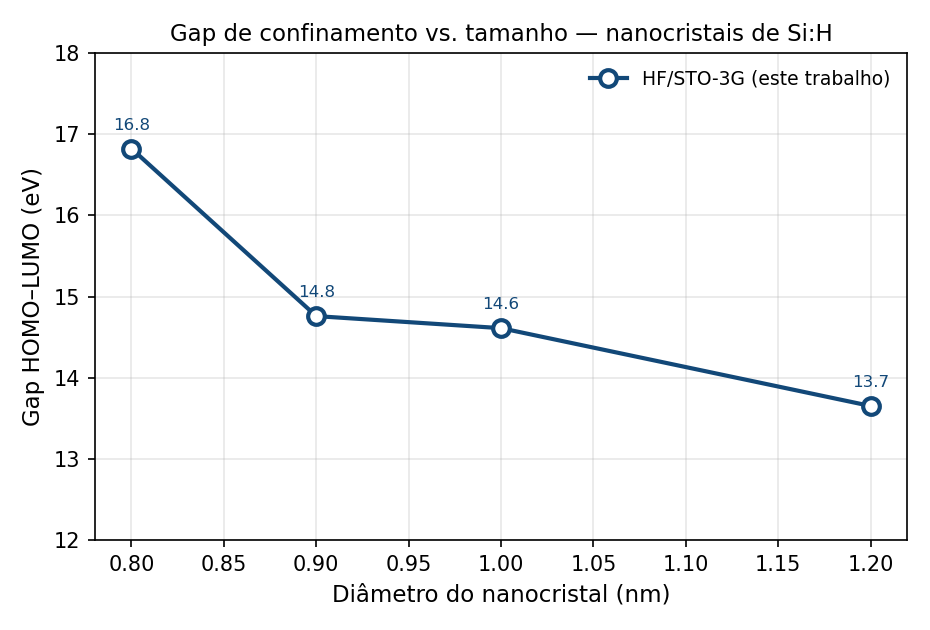
\includegraphics[width=0.78\textwidth]{figuras/gap_vs_tamanho.png}
  \caption{\emph{Gap} HOMO--LUMO calculado (HF/STO-3G) para nanocristais de Si:H
  em função do diâmetro. A queda monotônica com o tamanho é a assinatura do
  confinamento quântico. Os valores absolutos, porém, estão fortemente
  superestimados (ver texto).}
  \label{fig:gap}
\end{figure}

\begin{caixaatencao}
\textbf{A tendência é confiável; os valores absolutos, não.} Um leitor atento
estranhará: \emph{gaps} de $13$--$17$~eV? Nanocristais de Si desse tamanho exibem,
experimentalmente, \emph{gaps} ópticos de $3$--$4$~eV. Nosso cálculo os
superestima em cerca de quatro vezes --- e por bons motivos, todos instrutivos:
\begin{enumerate}[leftmargin=*,nosep]
  \item \textbf{Base mínima.} A STO-3G tem pouquíssimos orbitais virtuais, e eles
        ficam artificialmente altos, inflando o LUMO.
  \item \textbf{Ausência de correlação.} O Hartree-Fock ignora a correlação
        eletrônica e é notório por superestimar \emph{gaps}.
  \item \textbf{Orbitais virtuais de HF.} Os orbitais desocupados de HF sentem o
        potencial de $N$ elétrons (e não de $N-1$), o que os torna estimadores
        ruins de estados excitados.
\end{enumerate}
Isto não invalida o exercício --- pelo contrário. A \emph{física} (confinamento,
tendência com o tamanho) está correta; o que falha é a \emph{quantidade}. É
precisamente essa lacuna que motiva o Capítulo~5, onde a Teoria do Funcional da
Densidade e bases maiores nos aproximarão dos números experimentais.
\end{caixaatencao}

\subsection{O preço do realismo: o escalonamento na prática}

Ao rodar a varredura, você notará que os cálculos maiores demoram
desproporcionalmente mais. Na máquina em que este livro foi escrito, os tempos
foram: $\sim\!2$~s ($0{,}8$~nm, 106~funções), $17$~s ($0{,}9$~nm, 199), $27$~s
($1{,}0$~nm, 226) e $\sim\!8$~min ($1{,}2$~nm, 364). Quadruplicar o número de
funções de base multiplicou o tempo por mais de cem --- a assinatura do
escalonamento $N^4$ da Seção~\ref{sec:formalismo}. É por isso que o nanocristal
``oficial'' de $1{,}5$~nm (712~funções) do Projeto Âncora, embora perfeitamente
definível, exige paciência ou recursos de alto desempenho.

\begin{caixadica}
Para acelerar cálculos grandes, o \pyscf{} oferece o \emph{density fitting}, que
aproxima as integrais de dois elétrons e reduz drasticamente custo e memória:
\code{mf = scf.RHF(mol).density\_fit()}. O impacto na energia é pequeno; o ganho de
velocidade, enorme. Use-o sempre que o tamanho apertar.
\end{caixadica}

%---------------------------------------------------------------------
\begin{caixaancora}
\textbf{Etapa 1 --- O orbital do doador e o \emph{gap} eletrônico.}

Chegamos ao coração da Parte~I: localizar o \textbf{orbital que hospeda o
\qubit{}}. Diferentemente do silício puro (camada fechada), o sistema Si:P tem um
elétron desemparelhado. Num cálculo ROHF, isso se manifesta como um
\textbf{orbital simplesmente ocupado} (SOMO, \emph{Singly-Occupied Molecular
Orbital}): o estado do doador, com ocupação~1 em vez de~2 ou~0.

\vspace{0.2cm}
Por viabilidade computacional, executamos aqui o doador num nanocristal de
$1{,}0$~nm (Si$_{21}$P$_1$H$_{28}$, 337~elétrons); o de $1{,}5$~nm segue a mesma
receita, a custo maior.

\begin{lstlisting}[style=python]
import numpy as np
from pyscf import gto, scf
# reutiliza construir_nanocristal, inserir_doador, para_xyz do Capitulo 3

si, h = construir_nanocristal(1.0)
idx_p = inserir_doador(si)
mol = gto.M(atom=para_xyz(si, h, idx_p), basis='sto-3g', spin=1, verbose=0)

mf = scf.ROHF(mol)
mf.kernel()
assert mf.converged

# o SOMO e o orbital com ocupacao 1: o eletron do qubit
i_somo = int(np.where(mf.mo_occ == 1)[0][0])
print("SOMO: orbital #%d de %d, energia %.3f Ha"
      % (i_somo, len(mf.mo_occ), mf.mo_energy[i_somo]))

# quanto da densidade do SOMO esta localizada em torno do fosforo?
C = mf.mo_coeff[:, i_somo]
S = mol.intor('int1e_ovlp')
gross = C * (S @ C)                       # populacao por funcao de base
fatias = mol.aoslice_by_atom()
peso_atomo = np.array([gross[a[2]:a[3]].sum() for a in fatias])

iP = [mol.atom_symbol(i) for i in range(mol.natm)].index('P')
dist = np.linalg.norm(mol.atom_coords() - mol.atom_coords()[iP], axis=1) * 0.529
print("Densidade do SOMO sobre o P:        %.0f%%" % (100 * peso_atomo[iP]))
print("Densidade do SOMO ate 3 A do P:     %.0f%%" % (100 * peso_atomo[dist < 3].sum()))
\end{lstlisting}

\begin{lstlisting}[style=console]
SOMO: orbital #168 de 226, energia 0.157 Ha
Densidade do SOMO sobre o P:        19%
Densidade do SOMO ate 3 A do P:     83%
\end{lstlisting}

\textbf{O resultado que valida toda a Parte~I.} O orbital do \qubit{} não está
espalhado pelo nanocristal: \textbf{83\% de sua densidade concentra-se num raio de
$3$~Å em torno do fósforo}. O elétron excedente do doador está, de fato,
\emph{localizado} ao redor do P$^+$ --- é o ``hidrogênio artificial'' que a
intuição química do Capítulo~3 antecipou, agora confirmado por um cálculo de
primeiros princípios. É esse elétron localizado, e o seu spin, que
manipularemos como bit quântico.

\vspace{0.3cm}
\textbf{Sua tarefa.} No \emph{notebook} \code{projeto\_ancora\_SiP.ipynb}:
reproduza a varredura \emph{gap} vs.\ tamanho, gere a figura, e execute o cálculo
do doador acima. Registre: (a)~a energia do SOMO; (b)~o grau de localização;
(c)~por que a localização é essencial para um bom \qubit{} (dica: um estado
deslocalizado seria sensível a \emph{toda} a superfície e a suas imperfeições).

\vspace{0.3cm}
\textbf{A seguir.} No Capítulo~5, a Teoria do Funcional da Densidade corrigirá os
\emph{gaps} superestimados e nos dará acesso às propriedades ópticas do Si:P ---
antes de mergulharmos, na Parte~II, nos parâmetros magnéticos que definem o
\qubit{}: o acoplamento hiperfino e o tensor~\emph{g}.
\end{caixaancora}

%---------------------------------------------------------------------
\section*{Resumo do Capítulo}
\addcontentsline{toc}{section}{Resumo do Capítulo}
%---------------------------------------------------------------------

\begin{itemize}[leftmargin=*]
  \item O Hartree-Fock resolve as \textbf{equações de Roothaan-Hall}
        $\mathbf{FC} = \mathbf{SC}\boldsymbol{\varepsilon}$ de forma iterativa,
        porque a matriz de Fock depende da densidade que se quer obter --- o ciclo
        \textbf{SCF}.
  \item O custo escala como $N^4$ com o número de funções de base; por isso
        tamanho e base são sempre um compromisso, e o \emph{density fitting}
        (\code{.density\_fit()}) é um aliado valioso.
  \item A \textbf{convergência} é controlada por \emph{guess} inicial, DIIS,
        \code{level\_shift}, \code{max\_cycle} e \code{conv\_tol}. Sempre verifique
        \code{mf.converged} antes de usar resultados.
  \item O \textbf{gap} HOMO--LUMO de um ponto quântico é sua energia de
        confinamento: nossa varredura ($0{,}8$--$1{,}2$~nm) mostrou o \emph{gap}
        \textbf{diminuindo} com o tamanho, confirmando o confinamento quântico.
  \item Os valores absolutos de HF/STO-3G \textbf{superestimam} os \emph{gaps}
        (falta de correlação, base mínima, orbitais virtuais ruins) --- motivação
        para o DFT do Capítulo~5.
  \item \textbf{Projeto Âncora:} localizamos o \textbf{orbital do doador} (SOMO) no
        Si:P; \textbf{83\%} de sua densidade está a menos de $3$~Å do fósforo,
        confirmando o \qubit{} como um elétron localizado.
\end{itemize}

%---------------------------------------------------------------------
\section*{Exercícios}
\addcontentsline{toc}{section}{Exercícios}
%---------------------------------------------------------------------

\begin{enumerate}[leftmargin=*,label=\textbf{4.\arabic*}]
  \item \textbf{O ciclo SCF na prática.} Rode o nanocristal de $0{,}8$~nm com
        \code{verbose=4} e conte quantos ciclos o SCF levou para convergir. Depois
        aumente \code{mf.level\_shift} para $0{,}5$ e observe se o número de ciclos
        muda.

  \item \textbf{Verificando o escalonamento.} Cronometre (com o módulo \code{time})
        os cálculos de $0{,}8$, $0{,}9$ e $1{,}0$~nm. Faça um gráfico
        log--log do tempo contra \code{mol.nao} e estime o expoente do
        escalonamento. Ele se aproxima de~4?

  \item \textbf{Density fitting.} Repita o cálculo de $1{,}0$~nm com
        \code{scf.RHF(mol).density\_fit()} e compare energia total, \emph{gap} e
        tempo com o cálculo convencional. Valeu a pena?

  \item \textbf{Sensibilidade à base.} Recalcule o \emph{gap} do nanocristal de
        $0{,}8$~nm em STO-3G e em \code{6-31g}. O \emph{gap} sobe ou desce? Como
        isso se relaciona com a caixa de Atenção sobre valores absolutos?

  \item \textbf{O papel da passivação (revisão).} Construa o nanocristal de
        $0{,}8$~nm \emph{sem} passivar (sem hidrogênios) e tente rodar o SCF. Você
        provavelmente terá dificuldade de convergência ou um \emph{gap}
        minúsculo. Explique, com base nas ligações pendentes do Capítulo~3, o que
        aconteceu.

  \item \textbf{Projeto Âncora.} Para o doador Si:P de $1{,}0$~nm, examine também o
        orbital duplamente ocupado logo abaixo do SOMO e o primeiro virtual acima.
        Eles estão localizados no fósforo ou espalhados pelo nanocristal? O que
        isso diz sobre a natureza especial do estado do doador?
\end{enumerate}

%%=====================================================================
\chapter{Teoria do Funcional da Densidade: Corrigindo o \emph{Gap}}
\label{cap:dft}
%=====================================================================

O Capítulo~4 terminou com um incômodo produtivo. Nosso Hartree-Fock reproduziu
com fidelidade a \emph{física} do confinamento --- o \emph{gap} cai à medida que o
nanocristal cresce ---, mas errou a \emph{quantidade} por um fator de quatro:
\emph{gaps} de $13$--$17$~eV onde o experimento mede $3$--$4$~eV. A culpada tem
nome: a \textbf{correlação eletrônica}, que o Hartree-Fock ignora por construção.

Este capítulo apresenta a ferramenta que domina a química quântica moderna
justamente por incluir a correlação a um custo comparável ao do Hartree-Fock: a
\textbf{Teoria do Funcional da Densidade} (DFT, de \emph{Density Functional
Theory}). Veremos por que ela funciona, escolheremos um \emph{funcional} de troca
e correlação, e a colocaremos para trabalhar no \pyscf{}. Ao final, o \emph{gap}
do nosso ponto quântico terá encolhido para valores fisicamente razoáveis --- e,
como bônus, extrairemos a \textbf{densidade de spin} do doador, a grandeza que
abrirá a Parte~II do livro.

%---------------------------------------------------------------------
\section{Por Que o Hartree-Fock Não Basta}
\label{sec:porquedft}
%---------------------------------------------------------------------

Recordemos o pecado original do Hartree-Fock. Ele descreve cada elétron movendo-se
no \textbf{campo médio} de todos os outros, como se a nuvem eletrônica fosse um
borrão estático. A realidade é mais sutil: os elétrons, por se repelirem, executam
uma dança coordenada --- quando um se aproxima de certa região, os demais se
afastam. Essa correlação instantânea de seus movimentos \emph{abaixa} a energia do
sistema. A diferença entre a energia exata e a de Hartree-Fock é, por definição, a
\textbf{energia de correlação}:
\begin{equation}
  E_{\text{corr}} = E_{\text{exata}} - E_{\text{HF}} \;<\; 0.
  \label{eq:ecorr}
\end{equation}

\noindent
Em módulo, $E_{\text{corr}}$ costuma valer apenas $\sim 1\%$ da energia total ---
mas é justamente essa fração que governa as grandezas que nos interessam: energias
de ligação, barreiras de reação e, no nosso caso, o \emph{gap}. Ignorá-la, como
faz o Hartree-Fock, empurra sistematicamente os orbitais virtuais para cima e
infla o \emph{gap}.

\begin{caixanota}
\textbf{Duas rotas para a correlação.} A química quântica tem, historicamente,
dois caminhos para capturar $E_{\text{corr}}$. O primeiro são os métodos
\emph{pós-Hartree-Fock} (MP2, \emph{Coupled Cluster}, Interação de
Configurações), que partem da função de onda HF e a corrigem sistematicamente ---
precisos, porém caríssimos, com custos que escalam como $N^5$, $N^6$ ou pior.
Impensáveis para um nanocristal de centenas de elétrons. O segundo caminho, que
seguiremos, é o DFT: abandona a função de onda como objeto central e reformula
todo o problema em torno da \textbf{densidade eletrônica}, alcançando precisão
comparável a um custo próximo ao do próprio Hartree-Fock.
\end{caixanota}

%---------------------------------------------------------------------
\section{A Ideia Central: da Função de Onda à Densidade}
\label{sec:ideiadft}
%---------------------------------------------------------------------

A função de onda de $N$ elétrons, $\Psi(\mathbf{r}_1,\dots,\mathbf{r}_N)$, é um
objeto monstruoso: depende de $3N$ coordenadas espaciais. Para o nosso nanocristal
de mil elétrons, são três mil variáveis --- um objeto que nenhum computador jamais
armazenará por completo.

A DFT nasce de uma percepção revolucionária, formalizada em 1964 por
\textbf{Hohenberg e Kohn}: toda a informação do estado fundamental está contida na
humilde \textbf{densidade eletrônica} $\rho(\mathbf{r})$ --- a probabilidade de
encontrar um elétron em cada ponto do espaço. E $\rho$ depende de apenas
\textbf{três} coordenadas, $(x,y,z)$, não importa quantos elétrons existam. Os dois
teoremas de Hohenberg-Kohn garantem que:

\begin{enumerate}[leftmargin=*]
  \item A energia do estado fundamental é um \textbf{funcional único} da densidade,
        $E = E[\rho]$: conhecida $\rho(\mathbf{r})$, tudo o mais está determinado.
  \item Esse funcional atinge seu mínimo na densidade \emph{verdadeira} do estado
        fundamental --- fornecendo um princípio variacional para encontrá-la.
\end{enumerate}

\begin{caixanota}
\textbf{Funcional?} Uma \emph{função} recebe um número e devolve um número
($f(x) = x^2$). Um \textbf{funcional} recebe uma \emph{função inteira} e devolve um
número. A energia $E[\rho]$ é um funcional: alimenta-se com a função
$\rho(\mathbf{r})$ (definida em todo o espaço) e produz um único valor, a energia
em hartree. A notação com colchetes, $E[\rho]$, sinaliza essa distinção.
\end{caixanota}

O problema é que os teoremas garantem a \emph{existência} do funcional $E[\rho]$
mas não revelam sua \emph{forma}. Em especial, ninguém conhece a expressão exata
para a energia cinética em termos apenas de $\rho$. É aqui que entra a engenhosa
solução que tornou a DFT prática.

%---------------------------------------------------------------------
\section{As Equações de Kohn-Sham}
\label{sec:kohnsham}
%---------------------------------------------------------------------

Em 1965, \textbf{Kohn e Sham} deram o passo decisivo. Em vez de buscar a energia
cinética do sistema real de elétrons interagentes, eles introduziram um
\textbf{sistema auxiliar fictício} de elétrons \emph{não} interagentes, construído
para ter \textbf{exatamente a mesma densidade} $\rho(\mathbf{r})$ do sistema real.
Nesse sistema fictício, os elétrons ocupam orbitais --- os \textbf{orbitais de
Kohn-Sham} $\psi_i$ --- e a energia cinética se calcula trivialmente, como no
Hartree-Fock.

A densidade se reconstrói a partir desses orbitais,
\begin{equation}
  \rho(\mathbf{r}) = \sum_i^{\text{ocupados}} |\psi_i(\mathbf{r})|^2,
  \label{eq:rhoKS}
\end{equation}
e os orbitais obedecem a equações de aparência familiar, as \textbf{equações de
Kohn-Sham}:
\begin{equation}
  \left[ -\tfrac{1}{2}\nabla^2 + v_{\text{ext}}(\mathbf{r})
         + v_{\text{H}}[\rho](\mathbf{r})
         + v_{\text{xc}}[\rho](\mathbf{r}) \right] \psi_i
  = \varepsilon_i\,\psi_i.
  \label{eq:ks}
\end{equation}

\noindent
Os três primeiros termos são conhecidos e exatos: a energia cinética, a atração
$v_{\text{ext}}$ pelos núcleos e a repulsão eletrostática clássica $v_{\text{H}}$
(o potencial de Hartree). \textbf{Toda a nossa ignorância foi empurrada para o
último termo}, $v_{\text{xc}}$, o \textbf{potencial de troca e correlação}, derivado
do funcional $E_{\text{xc}}[\rho]$. Ele contém tudo o que é quântico e difícil: a
troca (a antissimetria de Pauli) \emph{e} a correlação que faltava ao
Hartree-Fock.

\begin{caixanota}
\textbf{A analogia com o SCF.} A Equação~\ref{eq:ks} é estruturalmente idêntica às
equações de Roothaan-Hall do Capítulo~4: um problema de autovalores em que o
operador depende da densidade, que depende dos orbitais, que dependem do operador.
Resolve-se, como o Hartree-Fock, por \textbf{iteração autoconsistente} --- o mesmo
ciclo SCF, com o mesmo \code{|ddm|} despencando a cada passo. A única novidade é a
troca do termo de troca exato de Fock pelo funcional $v_{\text{xc}}$. Por isso, do
ponto de vista do \pyscf{}, migrar de HF para DFT custará uma única linha de
código.
\end{caixanota}

\begin{caixaatencao}
\textbf{A DFT é exata --- na teoria.} As equações de Kohn-Sham seriam
\emph{exatas} se conhecêssemos o funcional $E_{\text{xc}}[\rho]$ verdadeiro. Mas
esse funcional universal é desconhecido, e talvez incognoscível em forma fechada.
Toda DFT prática usa uma \textbf{aproximação} para $E_{\text{xc}}$. É por isso que,
ao contrário do Coupled Cluster, a DFT não pode ser sistematicamente melhorada:
escolher um funcional melhor é uma arte guiada por física e validação, não uma
receita convergente. A próxima seção é sobre essa escolha.
\end{caixaatencao}

%---------------------------------------------------------------------
\section{A Escada de Jacob: Escolhendo o Funcional}
\label{sec:funcionais}
%---------------------------------------------------------------------

As aproximações para $E_{\text{xc}}$ são tradicionalmente organizadas na
\textbf{escada de Jacob}, uma metáfora de John Perdew: cada degrau incorpora mais
informação sobre a densidade, aproximando-se do ``céu'' da precisão química ao
preço de mais custo.

\begin{itemize}[leftmargin=*]
  \item \textbf{LDA} (\emph{Local Density Approximation}) --- o primeiro degrau.
        A energia de troca e correlação em cada ponto depende apenas da densidade
        \emph{local} $\rho(\mathbf{r})$, tomada como a de um gás uniforme de
        elétrons. Simples e surpreendentemente útil, mas superliga: erra energias
        de ligação por dezenas de kcal/mol.
  \item \textbf{GGA} (\emph{Generalized Gradient Approximation}) --- o segundo
        degrau. Acrescenta a \emph{inclinação} da densidade, o gradiente
        $\nabla\rho$, corrigindo boa parte dos excessos da LDA. O funcional
        \textbf{PBE} (Perdew-Burke-Ernzerhof) é o cavalo de batalha desta
        categoria, quase um padrão universal em física do estado sólido.
  \item \textbf{meta-GGA} --- o terceiro degrau, que ainda inclui a densidade de
        energia cinética (ex.: SCAN, TPSS).
  \item \textbf{Híbridos} --- o quarto degrau, que \emph{mistura} uma fração da
        troca exata de Hartree-Fock com a troca de um GGA. O célebre \textbf{B3LYP}
        (20\% de troca HF) domina a química molecular; o \textbf{PBE0} (25\%) é seu
        equivalente mais físico. Híbridos costumam dar os melhores \emph{gaps}, ao
        custo de reintroduzir as integrais de troca exata --- mais caras.
\end{itemize}

\begin{table}[h]
  \centering
  \caption{Degraus da escada de Jacob usados neste livro.}
  \label{tab:funcionais}
  \begin{tabular}{llll}
    \toprule
    \textbf{Degrau} & \textbf{Ingrediente} & \textbf{Exemplo} & \textbf{Custo} \\
    \midrule
    LDA      & $\rho$                      & LDA/SVWN & baixo \\
    GGA      & $\rho, \nabla\rho$          & PBE      & baixo \\
    meta-GGA & $+\,\tau$ (energia cinética) & SCAN     & médio \\
    Híbrido  & $+$ troca exata de HF        & B3LYP, PBE0 & alto \\
    \bottomrule
  \end{tabular}
\end{table}

\begin{caixadica}
\textbf{Qual escolher?} Para uma primeira estimativa rápida e barata, use
\textbf{PBE}: robusto, universal e sem parâmetros ajustados. Quando o alvo for o
\emph{gap} ou propriedades eletrônicas finas, suba um degrau e use um híbrido como
\textbf{B3LYP} ou \textbf{PBE0}. Neste capítulo compararemos os dois para ver, com
os próprios olhos, o efeito da troca exata sobre o \emph{gap} do ponto quântico.
\end{caixadica}

%---------------------------------------------------------------------
\section{DFT no PySCF: o Módulo \code{dft}}
\label{sec:dftpyscf}
%---------------------------------------------------------------------

A promessa da caixa de Nota da Seção~\ref{sec:kohnsham} agora se cumpre. Para o
\pyscf{}, trocar Hartree-Fock por DFT é substituir o módulo \code{scf} pelo módulo
\code{dft} e informar o funcional desejado no atributo \code{.xc}. Todo o resto ---
o objeto \Mole{}, o \code{kernel()}, a leitura de \code{mo\_energy} --- permanece
idêntico ao que já dominamos.

\begin{lstlisting}[style=python,caption={Um cálculo DFT em três linhas.},label={lst:rks}]
from pyscf import gto, dft

mol = gto.M(atom="H 0 0 0; H 0 0 0.74", basis='sto-3g')

mf = dft.RKS(mol)        # RKS = Restricted Kohn-Sham (camada fechada)
mf.xc = 'pbe'            # o funcional de troca e correlacao
energia = mf.kernel()

print("Energia PBE:", energia, "Ha")
\end{lstlisting}

\noindent
Onde antes escrevíamos \code{scf.RHF(mol)}, agora escrevemos \code{dft.RKS(mol)} e
acrescentamos a linha \code{mf.xc = 'pbe'}. A correspondência entre os métodos é
direta:

\begin{table}[h]
  \centering
  \caption{Correspondência entre os métodos de camada fechada e aberta.}
  \label{tab:hfvsks}
  \begin{tabular}{lll}
    \toprule
    \textbf{Camada} & \textbf{Hartree-Fock} & \textbf{Kohn-Sham (DFT)} \\
    \midrule
    Fechada (spin=0)        & \code{scf.RHF}  & \code{dft.RKS} \\
    Aberta, restrita        & \code{scf.ROHF} & \code{dft.ROKS} \\
    Aberta, irrestrita      & \code{scf.UHF}  & \code{dft.UKS} \\
    \bottomrule
  \end{tabular}
\end{table}

\subsection{A malha de integração}

Há uma diferença conceitual que vale mencionar. O termo $E_{\text{xc}}$ não pode ser
integrado analiticamente como as integrais de dois elétrons do Hartree-Fock; ele é
avaliado \textbf{numericamente}, sobre uma malha (\emph{grid}) de pontos que envolve
cada átomo. A densidade da malha controla a precisão:

\begin{lstlisting}[style=python,caption={Ajustando a malha de integração.},label={lst:grid}]
mf = dft.RKS(mol)
mf.xc = 'pbe'
mf.grids.level = 3       # 0 (grosseira) a 9 (finissima); padrao = 3
energia = mf.kernel()
\end{lstlisting}

\begin{caixaatencao}
\textbf{A malha pode trair você.} Uma malha grosseira demais introduz ``ruído
numérico'' na energia, chegando a impedir a convergência do SCF ou a produzir
diferenças de energia sem sentido físico. O padrão \code{grids.level = 3} é
adequado para a maioria dos casos; se um cálculo DFT oscilar ou der energias
irreprodutíveis, \textbf{aumente a malha} antes de suspeitar de qualquer outra
coisa. O custo extra costuma valer a tranquilidade.
\end{caixaatencao}

\begin{caixadica}
Os nomes de funcionais no \pyscf{} são \emph{strings} e cobrem centenas de opções
via a biblioteca \emph{Libxc}. Os mais usados: \code{'lda'}, \code{'pbe'},
\code{'b3lyp'}, \code{'pbe0'}, \code{'scan'}. É possível até combinar componentes
manualmente (ex.: \code{mf.xc = '0.2*HF + 0.8*B88, LYP'}), mas para nós os nomes
prontos bastam. Consulte \code{dft.libxc.XC\_CODES} para a lista completa.
\end{caixadica}

%---------------------------------------------------------------------
\section{Mãos à Obra: Hartree-Fock \emph{versus} DFT no \emph{Gap}}
\label{sec:maos5}
%---------------------------------------------------------------------

Chegou a hora de saldar a dívida do Capítulo~4. Vamos recalcular o \emph{gap} dos
mesmos nanocristais de silício, agora com PBE e B3LYP, e confrontar os três métodos
lado a lado. A previsão é clara: a correlação deve \textbf{fechar} o \emph{gap}
inflado do Hartree-Fock.

\begin{caixamaos}
\textbf{Objetivo:} calcular o \emph{gap} HOMO--LUMO dos nanocristais de Si:H com
HF, PBE e B3LYP, e comparar a queda provocada pela correlação.

\begin{lstlisting}[style=python]
import numpy as np
from pyscf import gto, scf, dft
# reutiliza construir_nanocristal e para_xyz do Capitulo 3

def gap_homo_lumo(mf):
    """Gap HOMO-LUMO (eV) de um objeto SCF/KS de camada fechada ja convergido."""
    no = int(mf.mo_occ.sum() // 2)
    return (mf.mo_energy[no] - mf.mo_energy[no - 1]) * 27.2114

def calcula_gaps(diametro):
    si, h = construir_nanocristal(diametro)
    mol = gto.M(atom=para_xyz(si, h), basis='sto-3g', verbose=0)

    hf = scf.RHF(mol);           hf.kernel()
    pbe = dft.RKS(mol);   pbe.xc = 'pbe';   pbe.kernel()
    b3 = dft.RKS(mol);    b3.xc = 'b3lyp';  b3.kernel()
    assert hf.converged and pbe.converged and b3.converged
    return gap_homo_lumo(hf), gap_homo_lumo(pbe), gap_homo_lumo(b3)

print("  D(nm)     HF     PBE   B3LYP")
for d in [0.8, 0.9, 1.0, 1.2]:
    g_hf, g_pbe, g_b3 = calcula_gaps(d)
    print("  %4.1f  %6.2f  %6.2f  %6.2f" % (d, g_hf, g_pbe, g_b3))
\end{lstlisting}

\begin{lstlisting}[style=console]
  D(nm)     HF     PBE   B3LYP
   0.8   16.82    8.29    9.86
   0.9   14.76    6.77    8.23
   1.0   14.61    6.66    8.11
   1.2   13.65    5.99    7.37
\end{lstlisting}
\end{caixamaos}

\noindent
O resultado é eloquente. A Tabela~\ref{tab:gapmetodos} reúne os números. Para o
nanocristal de $0{,}8$~nm, o \emph{gap} cai de $16{,}82$~eV (HF) para $8{,}29$~eV
(PBE) --- uma redução para praticamente metade. O B3LYP, que reintroduz $20\%$ da troca
exata de Hartree-Fock, situa-se \textbf{entre} os dois extremos, exatamente como a
teoria previa: mais troca exata, maior o \emph{gap}.

\begin{table}[h]
  \centering
  \caption{\emph{Gap} HOMO--LUMO (eV) de nanocristais de Si:H por três métodos
  (base STO-3G). A correlação capturada pela DFT reduz drasticamente a
  superestimativa do Hartree-Fock.}
  \label{tab:gapmetodos}
  \begin{tabular}{lcccc}
    \toprule
    \textbf{Diâmetro} & \textbf{HF} & \textbf{PBE} & \textbf{B3LYP}
                      & \textbf{Tendência} \\
    \midrule
    $0{,}8$~nm & $16{,}82$ & $8{,}29$ & $9{,}86$ & \multirow{4}{*}{$\searrow$ com o tamanho} \\
    $0{,}9$~nm & $14{,}76$ & $6{,}77$ & $8{,}23$ & \\
    $1{,}0$~nm & $14{,}61$ & $6{,}66$ & $8{,}11$ & \\
    $1{,}2$~nm & $13{,}65$ & $5{,}99$ & $7{,}37$ & \\
    \bottomrule
  \end{tabular}
\end{table}

\noindent
E, crucialmente, os três métodos preservam a \textbf{tendência} do confinamento: o
\emph{gap} cai monotonicamente com o tamanho em todos eles. A física estava certa
desde o Capítulo~4; a DFT apenas ajustou a escala. Um gráfico sobrepondo as três
curvas torna o quadro imediato:

\begin{lstlisting}[style=python]
import matplotlib.pyplot as plt

diametros = [0.8, 0.9, 1.0, 1.2]
resultados = np.array([calcula_gaps(d) for d in diametros])   # colunas: HF, PBE, B3LYP

for coluna, nome, marca in zip(range(3), ["HF", "PBE", "B3LYP"], ["s--", "o-", "^-"]):
    plt.plot(diametros, resultados[:, coluna], marca, label=nome)
plt.xlabel("Diametro (nm)"); plt.ylabel("Gap HOMO-LUMO (eV)")
plt.legend(); plt.grid(alpha=0.3); plt.show()
\end{lstlisting}

\begin{caixaatencao}
\textbf{O \emph{gap} de Kohn-Sham não é o \emph{gap} óptico.} Reduzimos a
superestimativa do Hartree-Fock, mas o leitor rigoroso deve saber: a diferença
$\varepsilon_{\text{LUMO}} - \varepsilon_{\text{HOMO}}$ dos orbitais de Kohn-Sham é
uma grandeza \emph{do estado fundamental}, e não corresponde exatamente à energia
de uma excitação óptica real (que envolve, ademais, a atração entre o elétron
excitado e o buraco que ele deixa). O \emph{gap} óptico rigoroso exige a
\textbf{DFT dependente do tempo} (TDDFT), assunto de um volume futuro. Some-se a
isso a base mínima STO-3G, que ainda infla os virtuais. Nosso objetivo aqui é mais
modesto e legítimo: mostrar que a \textbf{correlação move os números na direção
certa}, aproximando-os da faixa experimental de $3$--$4$~eV. E move --- de forma
espetacular.
\end{caixaatencao}

%---------------------------------------------------------------------
\begin{caixaancora}
\textbf{Etapa 2 --- O \emph{gap} corrigido e a densidade de spin do doador.}

Com a DFT em mãos, revisitamos o sistema Si:P do Capítulo~4 --- desta vez com
camada aberta irrestrita (\code{dft.UKS}), o método que dá a cada spin sua própria
densidade e, por isso, acessa diretamente a grandeza que definirá o \qubit{}: a
\textbf{densidade de spin} $\rho_\uparrow(\mathbf{r}) - \rho_\downarrow(\mathbf{r})$,
a assinatura espacial do elétron desemparelhado.

\begin{lstlisting}[style=python]
import numpy as np
from pyscf import gto, dft
# reutiliza construir_nanocristal, inserir_doador, para_xyz do Capitulo 3

si, h = construir_nanocristal(1.0)
idx_p = inserir_doador(si)
mol = gto.M(atom=para_xyz(si, h, idx_p), basis='sto-3g', spin=1, verbose=0)

mf = dft.UKS(mol)
mf.xc = 'pbe'
mf.kernel()
assert mf.converged

# densidade de spin projetada em cada atomo (analise de Mulliken)
dma, dmb = mf.make_rdm1()                 # matrizes de densidade alfa e beta
S = mol.intor('int1e_ovlp')
spin_ao = np.einsum('ij,ji->i', dma - dmb, S)   # spin liquido por funcao de base
fatias = mol.aoslice_by_atom()
spin_atomo = np.array([spin_ao[a[2]:a[3]].sum() for a in fatias])

iP = [mol.atom_symbol(i) for i in range(mol.natm)].index('P')
dist = np.linalg.norm(mol.atom_coords() - mol.atom_coords()[iP], axis=1) * 0.529

print("Spin total integrado:            %.2f" % spin_atomo.sum())
print("Densidade de spin sobre o P:     %.0f%%" % (100 * spin_atomo[iP]))
print("Densidade de spin ate 3 A do P:  %.0f%%" % (100 * spin_atomo[dist < 3].sum()))
\end{lstlisting}

\begin{lstlisting}[style=console]
Spin total integrado:            1.00
Densidade de spin sobre o P:     12%
Densidade de spin ate 3 A do P:  80%
\end{lstlisting}

\textbf{A física do \qubit{}, agora em cores de spin.} O spin líquido integra a
exatamente~1 --- há um, e apenas um, elétron desemparelhado, como manda a contagem
ímpar do Capítulo~3. E ele não está espalhado: \textbf{80\% da densidade de spin
concentra-se num raio de $3$~Å em torno do fósforo}, corroborando com um método
correlacionado o que o SOMO de Hartree-Fock já havia sugerido. O elétron do doador
é, de fato, um ``átomo de hidrogênio artificial'' ancorado ao caroço P$^+$.

\vspace{0.3cm}
\textbf{Por que a densidade de spin é o próximo tesouro.} Essa não é uma grandeza
qualquer. É a densidade de spin \emph{no próprio núcleo} de $^{31}$P que determina
o \textbf{acoplamento hiperfino de contato de Fermi} --- o diálogo entre o spin do
elétron (nosso \qubit{}) e o spin do núcleo, e um dos parâmetros mais importantes
de um \qubit{} de spin em silício. Acabamos de calcular, pela primeira vez no
livro, o objeto de onde esse acoplamento brota. A Parte~II inteira se dedicará a
extraí-lo com rigor.

\vspace{0.3cm}
\textbf{Sua tarefa.} No \emph{notebook} \code{projeto\_ancora\_SiP.ipynb}:
\begin{enumerate}[leftmargin=*,nosep]
  \item Reproduza a tabela HF/PBE/B3LYP do \emph{gap} (Tabela~\ref{tab:gapmetodos})
        e gere o gráfico sobreposto das três curvas.
  \item Execute o cálculo \code{dft.UKS} do doador de $1{,}0$~nm e registre a
        densidade de spin sobre o P e dentro de $3$~Å.
  \item Numa célula de texto, explique com suas palavras: (a)~por que a DFT reduz o
        \emph{gap} em relação ao HF; (b)~por que a localização da densidade de spin
        no fósforo é uma boa notícia para a estabilidade do \qubit{}.
\end{enumerate}

\vspace{0.3cm}
\textbf{A seguir.} Encerramos a Parte~I com uma imagem completa da estrutura
eletrônica do nosso ponto quântico: geometria (Cap.~3), orbitais e \emph{gap}
(Cap.~4) e agora um \emph{gap} corrigido pela correlação, além da densidade de spin
do doador (Cap.~5). A Parte~II dará o salto seguinte --- transformar essa densidade
de spin nos \textbf{parâmetros magnéticos} que caracterizam o \qubit{}: o
acoplamento hiperfino e o tensor~\emph{g}.
\end{caixaancora}

%---------------------------------------------------------------------
\section*{Resumo do Capítulo}
\addcontentsline{toc}{section}{Resumo do Capítulo}
%---------------------------------------------------------------------

\begin{itemize}[leftmargin=*]
  \item O Hartree-Fock ignora a \textbf{correlação eletrônica}
        ($E_{\text{corr}} = E_{\text{exata}} - E_{\text{HF}} < 0$), o que infla
        sistematicamente os \emph{gaps}.
  \item A \textbf{DFT} reformula o problema em torno da densidade
        $\rho(\mathbf{r})$, que depende de apenas 3 coordenadas. Os teoremas de
        \textbf{Hohenberg-Kohn} garantem que $E = E[\rho]$ e que $\rho$ é
        variacional.
  \item As \textbf{equações de Kohn-Sham} têm a mesma estrutura iterativa (SCF) do
        Hartree-Fock; toda a dificuldade reside no \textbf{funcional de troca e
        correlação} $E_{\text{xc}}[\rho]$, que é aproximado.
  \item A \textbf{escada de Jacob} organiza os funcionais: LDA
        ($\rho$) $\to$ GGA/PBE ($\nabla\rho$) $\to$ meta-GGA $\to$ híbridos
        (B3LYP, PBE0, com troca exata).
  \item No \pyscf{}, DFT é o módulo \code{dft}: \code{dft.RKS}/\code{ROKS}/\code{UKS},
        com \code{mf.xc = 'pbe'} (ou \code{'b3lyp'}) e a malha \code{mf.grids.level}.
  \item Na prática, PBE e B3LYP \textbf{reduziram o \emph{gap}} do nanocristal de
        Si:H em relação ao HF (de $\sim\!17$ para $\sim\!6$~eV a $0{,}8$~nm),
        preservando a tendência de confinamento --- embora o \emph{gap} de
        Kohn-Sham ainda não seja o \emph{gap} óptico (TDDFT).
  \item \textbf{Projeto Âncora:} com \code{dft.UKS}, obtivemos a \textbf{densidade
        de spin} do doador, localizada ($\sim\!80\%$ a menos de $3$~Å do P) --- a
        semente do acoplamento hiperfino que a Parte~II calculará.
\end{itemize}

%---------------------------------------------------------------------
\section*{Exercícios}
\addcontentsline{toc}{section}{Exercícios}
%---------------------------------------------------------------------

\begin{enumerate}[leftmargin=*,label=\textbf{5.\arabic*}]
  \item \textbf{HF é DFT?} Explique, em duas ou três frases, por que o Hartree-Fock
        pode ser visto como um caso particular das equações de Kohn-Sham. Qual
        termo de $E_{\text{xc}}$ ele inclui e qual ele omite?

  \item \textbf{O efeito do funcional.} Para o nanocristal de $0{,}8$~nm, calcule o
        \emph{gap} com \code{'lda'}, \code{'pbe'} e \code{'pbe0'}. Ordene os
        funcionais pelo \emph{gap} que produzem e relacione a ordem à fração de
        troca exata de cada um.

  \item \textbf{A malha importa.} Rode o nanocristal de $0{,}9$~nm com PBE variando
        \code{mf.grids.level} de $1$ a $5$. A partir de qual nível a energia total
        estabiliza (varia menos de $10^{-4}$~Ha)? Que nível você recomendaria como
        compromisso?

  \item \textbf{Correlação em números.} Para o nanocristal de $0{,}8$~nm, calcule a
        energia total em HF e em PBE. A diferença é uma estimativa (grosseira) da
        energia de correlação. Que fração da energia total ela representa? Confere
        com o ``$\sim 1\%$'' mencionado no texto?

  \item \textbf{Restrito vs.\ irrestrito.} Repita o cálculo do doador Si:P de
        $1{,}0$~nm com \code{dft.ROKS} e com \code{dft.UKS} (ambos com PBE). Compare
        a energia total e o valor de \code{mf.spin\_square()}. O UKS sofre de
        \emph{contaminação de spin}? O que $\langle S^2\rangle$ deveria valer
        idealmente para um dubleto?

  \item \textbf{Projeto Âncora.} Refaça a Etapa~2 trocando PBE por B3LYP no cálculo
        \code{dft.UKS} do doador. A densidade de spin sobre o fósforo muda muito? O
        que isso sugere sobre a robustez da localização do \qubit{} frente à
        escolha do funcional?
\end{enumerate}


% ---------------- Parte II: Parametros Magneticos --------------------
%\input{tex/parte2}
%\input{tex/cap06_hiperfino}
%\input{tex/cap07_tensor_g}

% ---------------- Parte III: Dois Qubits e Coerencia -----------------
%\input{tex/parte3}
%\input{tex/cap08_troca}
%\input{tex/cap09_decoerencia}

% ---------------- Parte IV: Controlando o Qubit ----------------------
%\input{tex/parte4}
%\input{tex/cap10_stark}

% ---------------- Parte V: Do Qubit ao Dispositivo -------------------
%\input{tex/parte5}
%\input{tex/cap11_multiescala}

%\input{tex/cap12_consolidacao}

\end{document}
